\documentclass[review]{elsarticle}

\usepackage{lineno,hyperref}
\usepackage[utf8]{inputenc}
\usepackage{graphicx}
\usepackage{amsfonts}
\usepackage{mathtools}
\usepackage{tikz}
\usetikzlibrary{shapes,arrows,chains,calc}

% Set up a few colours for tikz figure
\colorlet{lcfree}{green}
\colorlet{lcnorm}{blue}
\colorlet{lccong}{red}



\modulolinenumbers[5]

\journal{Ecological Modelling}

%%%%%%%%%%%%%%%%%%%%%%%
%% Elsevier bibliography styles
%%%%%%%%%%%%%%%%%%%%%%%
%% To change the style, put a % in front of the second line of the current style and
%% remove the % from the second line of the style you would like to use.
%%%%%%%%%%%%%%%%%%%%%%%

%% Numbered
%\bibliographystyle{model1-num-names}
%% Numbered without titles
%\bibliographystyle{model1a-num-names}
%% Harvard
%%\bibliographystyle{model2-names.bst}\biboptions{authoryear}
%% Vancouver numbered
%\usepackage{numcompress}\bibliographystyle{model3-num-names}
%% Vancouver name/year
%\usepackage{numcompress}\bibliographystyle{model4-names}\biboptions{authoryear}
%% APA style
%%\bibliographystyle{model5-names}\biboptions{authoryear}
%% AMA style
%\usepackage{numcompress}\bibliographystyle{model6-num-names}
%% `Elsevier LaTeX' style
\bibliographystyle{elsarticle-num}
%%%%%%%%%%%%%%%%%%%%%%%

\begin{document}

\begin{frontmatter}

\title{A simulation framework for exploring spatio-temporal dynamics in mixed
	fisheries}

%% Group authors per affiliation:
\author[1,2]{Paul J. Dolder\corref{c}}
\cortext[c]{Corresponding author}
\ead{paul.dolder@gmit.ie}

\author[1]{Cóilín Minto}
\author[3]{Jean-Marc Guarini}
\author[4]{Jan-Jaap Poos}

\address[1]{Galway-Mayo Institute of Technology (GMIT), Dublin Road, Galway,
	Ireland} 
\address[2]{Centre for Environment, Fisheries and Aquaculture Science (Cefas),
	Pakefield Road, Lowestoft, UK}
\address[3]{Université Pierre et Marie Curie, 4 Place Jussieu, 75005 Paris,
	France}
\address[4]{Wageningen Marine Research, Haringkade 1 1976 CP IJmuiden,
	Netherlands}

\begin{abstract}
[A concise and factual abstract is required. The abstract should state briefly
the purpose of the research, the principal results and major conclusions. An
abstract is often pnresented separately from the article, so it must be able to
stand alone. For this reason, References should be avoided, but if essential,
then cite the author(s) and year(s). Also, non-standard or uncommon
abbreviations should be avoided, but if essential they must be defined at their
first mention in the abstract itself.  
Graphical abstract: Although a graphical abstract is optional, its use is
encouraged as it draws more attention to the online article. The graphical
abstract should summarize the contents of the article in a concise, pictorial
form designed to capture the attention of a wide readership. Graphical
abstracts should be submitted as a separate file in the online submission
system. Image size: Please provide an image with a minimum of 531 X 1328 pixels
(h X w) or proportionally more. The image should be readable at a size of 5 x
13 cm using a regular screen resolution of 96 dpi.  Preferred file types: TIFF,
EPS, PDF or MS Office files.]
\end{abstract}

\begin{keyword}
Some\sep keywords \sep here. Max 6, American "spelling" 
\MSC[2010] 00-01\sep  99-00
\end{keyword}

\end{frontmatter}

\linenumbers

\section{Introduction}

[Guidance:: State the objectives of the work and provide an adequate
background, avoiding a detailed literature survey or a summary of the results.]
\\

Fishers exploit fish populations that are heterogenously distributed in space
and time without prior knowledge of species distributions and non-selective
fishing gear. Fisheries managed by single-species quotas catch an assemblage of
species, known as mixed fisheries, leading to discarding of overquota catch.
Reducing discarding is crucial to ensure biological and economic sustainability
of fisheries. As such there is increasing interest in technical solutions
such as gear, spatial closures as a way of avoiding discarding unwanted catch.
\\

Use of spatial management as a tool is hampered by lack of knowledge of fish
and fishery spatiotemporal dyanmics and understanding of the scale at which
processes are important for management. Understanding of the correct scale for
spatial management is crucial in order to implement measures at a resolution
that ensures effective management\cite{Dunn2016} while minimising economic
impact; for example a scale which promote species avoidance for vulnerable or
low quota species while allowing continance of sustainable fisheries for
available quota species. \\

Ensuring measures are implemented at an appropriate scale has been a challenge
in the a past that has led to ineffectual measures with unitended consequences
such as limited impact towards the management objective or increased benthic
impact on previously unexploited areas (e.g. the cod closure in the North
Sea\cite{Rijnsdorp2001,Dinmore2003}). Since then more refined spatial
information has become available through the combination of logbook and Vessel
Monitoring System (VMS) data\cite{Lee2010, Bastardie2010, Gerritsen2012,
	Mateo2016}, though such information is patchy and derived from an
inherently biased sampling programme (i.e. targeted fishing). Further,
generally fishers only recorded landings (not catch) on a daily basis. This
leads to questions about the validity of inferences that can be drawn from
landings data assigned to VMS activity pings. \\ 

In order to test the assumption that VMS associated landings data can be used
to draw inference on the underlying population structures we develop a
simulation model where population dynamics are known rather than inferred from
sampling or commercial catches. Population movement is driven by a random
(diffusive) and directed (advective) process and we incorporate
characterisation of a number of different fisheries exploiting four fish
populations with different spatial and population demographics.\\

Using our model we simulation 20 years of exploitation of the fish populations
and use the results from the fishing model to draw inference on the underlying
population structures.  We compare this inference to i) a simulated
[stratified] fixed-site sampling design commonly used for fisheries monitoring
purposes, ii) the underlying population structures input to the simulation.\\

[Could fit a geostatistical model (e.g. VAST) to the fisheries-dependent and
fisheries-independent data, though may be overkill...] \\

We simulate a fishery closure to protect one species based on the
fishery-dependent inferred distributions at a spatial and temporal scale
typical in fisheries management, and assess a theoretical "benefit" to the
population, and effect on the other three populations. Further, we extend our
analysis to a range of spatial and temporal scales to assess the impact of
these processes on the success of the management measure. \\

\section{Materials and Methods}

[Guidance: Provide sufficient details to allow the work to be reproduced by an
independent researcher. Methods that are already published should be
summarized, and indicated by a reference.  If quoting directly from a
previously published method, use quotation marks and also cite the source. Any
modifications to existing methods should also be described.] \\ 

We develop a simulation model with a modular event-based approach, where
modules occur on independent time-scales appropriate to capture the
characteristic of the process modelled. The fishing model operated on a
tow-by-tow basis, while population dynamics (fishing and natural mortality,
growth) operate on a daily time-step.  Population movement occurs on a
two-weekly time-step, while recruitment occurs periodcally each year for a set
time period (e.g. 3 weeks) at at specified point individual to a species. The
model structure is summerised in Figure 1.\\

In the following section, we describe each of the model components; 1)
Population dynamics, 2) Recruitment dynamics, 3) Population movement, 4)
fishery dynamics.\\

%%%%%%%%%%%%%%%%%%%%%%%%%%%%%%%%%%%
% Overview schematic  
\begin{figure}[!ht]
	\hspace{-4em}
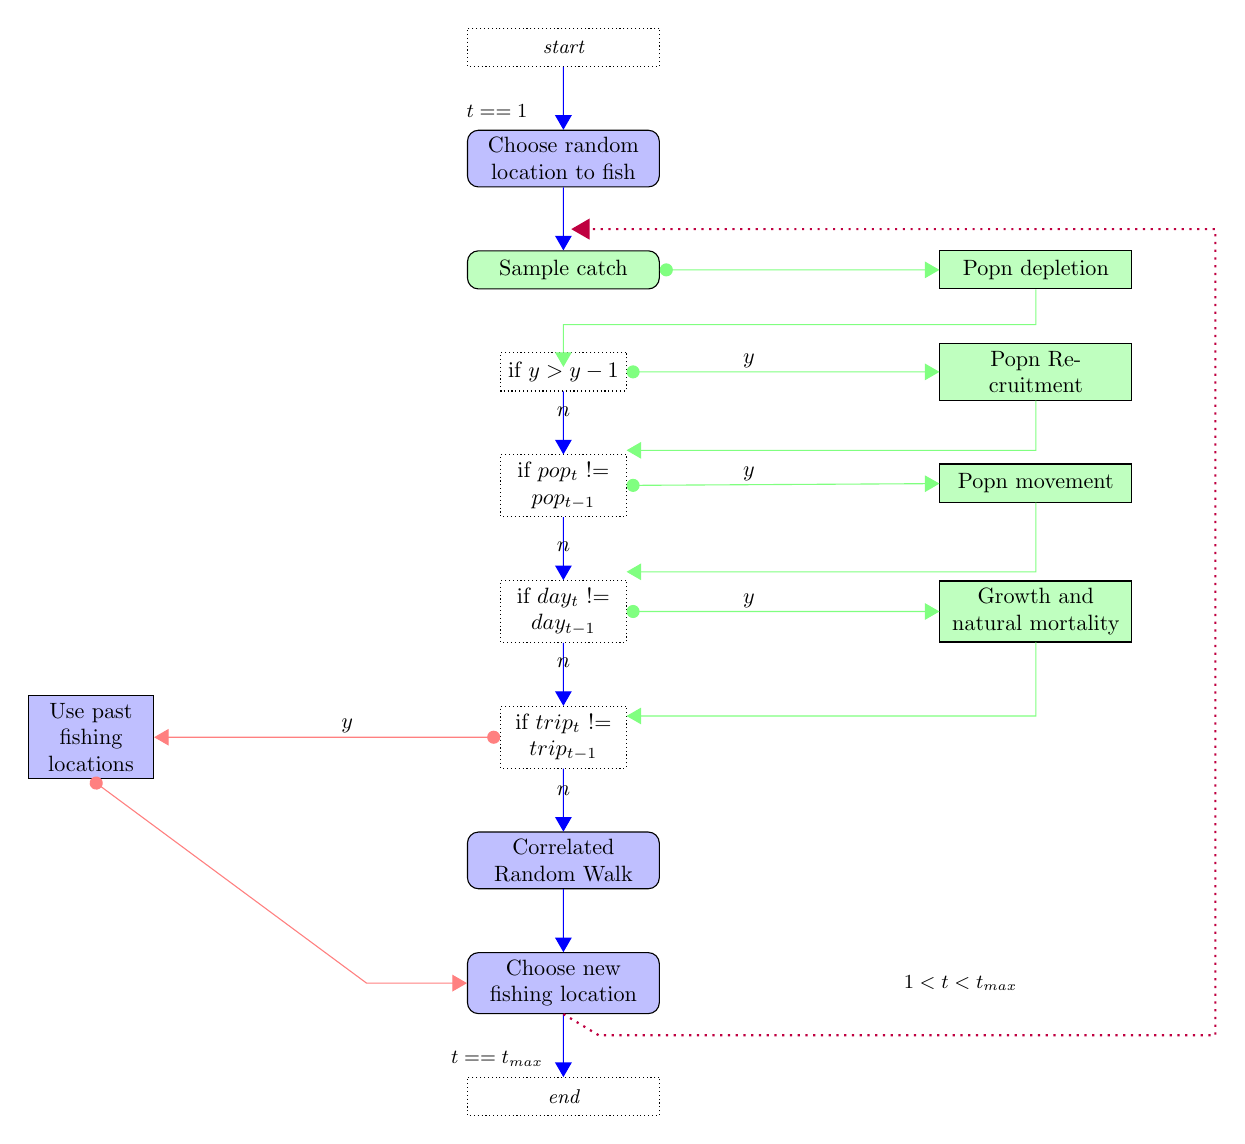
\begin{tikzpicture}[%
    >=triangle 60,              % Nice arrows; your taste may be different
    start chain=going below,    % General flow is top-to-bottom
    node distance=8mm and 60mm, % Global setup of box spacing
    every join/.style={norm},   % Default linetype for connecting boxes
    scale=0.9,
    every node/.style={scale=0.8}]                 
    \label{fig:model}
    % ------------------------------------------------- 
% A few box styles 
% <on chain> *and* <on grid> reduce the need for manual relative
% positioning of nodes
\tikzset{
  base/.style={draw, on chain, on grid, align=center, minimum height=4ex},
  proc/.style={base, rectangle, text width=8em},
  test/.style={base, rectangle, text width=5em},
  term/.style={proc, rounded corners},
  % coord node style is used for placing corners of connecting lines
  coord/.style={coordinate, on chain, on grid, node distance=6mm and 25mm},
  % nmark node style is used for coordinate debugging marks
  nmark/.style={draw, cyan, circle, font={\sffamily\bfseries}},
  % -------------------------------------------------
  % Connector line styles for different parts of the diagram
  norm/.style={->, draw, lcnorm},
  free/.style={->, draw, lcfree},
  cong/.style={->, draw, lccong},
  it/.style={font={\small\itshape}}
}
% -------------------------------------------------
% Start by placing the nodes in the middle
\node [proc, densely dotted, it] (p0) {start};
% Use join to connect a node to the previous one 
\node [term, join, fill=lcnorm!25]      {Choose random location to fish};
\node [term, join, fill=lcfree!25] (p1){Sample catch};
\node [test, densely dotted] (t1) {if $y > y-1$};
\node [test, join, densely dotted] (t2) {if $pop_{t}$ != $pop_{t-1}$};
\node [test, join, densely dotted] (wk) {if $day_{t}$ != $day_{t-1}$};
\node [test, join, densely dotted] (t3) {if $trip_{t}$ != $trip_{t-1}$};
\node [term, join, fill=lcnorm!25]  (p2) {Correlated Random Walk};
\node [term, join, fill=lcnorm!25]  (p3) {Choose new fishing location};
\node [proc, densely dotted, join, it] (p7) {end};

% Right nodes
\node [proc, fill=lcfree!25, right=of p1] (p4) {Popn depletion};
\node [proc, fill=lcfree!25, right=of t1] (p5) {Popn Recruitment};
\node [proc, fill=lcfree!25] (p6) {Popn movement};
\node [proc, fill=lcfree!25, right=of wk] (wk1) {Growth and natural
	mortality};

% left nodes
\node [test, fill=lcnorm!25, left=of t3] (t4) {Use past fishing locations};

% -------------------------------------------------
% A couple of boxes have annotations
\node [below=of p0, it, yshift=1.5em,xshift=-3em] {$t==1$};
\node [right=30mm of p3, it] {$1 < t < t_{max}$};
\node [below=of p3, it,xshift=-3em, yshift=1.5em] {$t == t_{max}$};

% -------------------------------------------------
% First, the straight north-south connections. In each case, we first
% draw a path with a (consistently positioned) annotation node, then
% we draw the arrow itself.
  \draw [*->,lcfree!50] (p1) -- (p4);
\path (t1) to node [near start, xshift=2em, yshift=0.5em] {$y$} (p5); 
  \draw [*->,lcfree!50] (t1) -- (p5);
\path (t2) to node [near start, xshift=2em, yshift=0.5em] {$y$} (p6); 
  \draw [*->,lcfree!50] (t2) -- (p6);
\path (t3) to node [near start, xshift=-3em, yshift=0.5em] {$y$} (t4); 
  \draw [*->,lccong!50] (t3) -- (t4);
\path (wk) to node [near start, xshift=2em, yshift=0.5em] {$y$} (wk1); 
  \draw [*->,lcfree!50] (wk) -- (wk1);

% left to right paths
\path (t1) to node [near start, yshift=-0.2em] {$n$} (t2) ;  
\path (t2) to node [near start, yshift=0.8em] {$n$} (t3) ;  
\path (wk) to node [near start, yshift=-0.2em] {$n$} (t3) ;  
\path (t3) to node [near start, yshift=-0.3em] {$n$} (p2) ;  

% ------------------------------------------------- 
% the twisty connectors. Again, we place the annotation
% first, then draw the connector

\node [coord, left=of p3] (c1)  {};  
\draw [*->,lccong!50] (t4.south) -- (c1) |- (p3);

\node[coord, below=of p4] (c2) {};
\node[coord, above=of t1] (c3) {};
\draw [-<,lcfree!50] (p4.south) -- (c2) |- (c3) |- (t1.north);

\node[coord, below=of p5] (c4) {};
\draw [->,lcfree!50] (p5.south) -- (c4) |- ($(t2.east) + (0,0.5)$);

\node[coord, below=of p6] (c71) {};
\draw [->,lcfree!50] (p6.south) -- (c71) |- ($(wk.east) + (0,0.56)$);

\node[coord, below=of wk1] (c7) {};
\draw [->,lcfree!50] (wk1.south) -- (c7) |- ($(t3.east) + (0,0.3)$);

% -------------------------------------------------
% A last flourish which breaks all the rules
\draw [->,purple, dotted, thick, shorten >=1mm]
  (p3.south) -- ++(5mm,-3mm)  -- ++(87mm,0mm) 
  |- node [black, near end, yshift=1.75em, it]
    {} ($(p1.north) + (0,0.3)$);
% -------------------------------------------------
\end{tikzpicture}
\caption{Overview Schematic of simulation model}
\end{figure}
%%%%%%%%%%%%%%%%%%%%%%%%%%

\subsection{Population dynamics}

The basic population level processes are simulated using a modified two-stage
Deriso-Schnute delay difference model \cite{Deriso1980, Schnute1985,
	Dichmont2003} occurring at a daily time-step. Here, population biomass
growth and depletion for pre-recruits and fish recruited to the fishery are
modelled separately as a function of previous recruited biomass, intrinsic
population growth and recruitment:

\begin{equation*}
	\begin{split}
	B_{y,w+1} = &\\
	& (1 + \rho) B_{y,w} \cdot e^{-Z_{y,w}} - \rho \cdot e^{-Z_{y,w}} \hspace{2.9cm}
	\times \\  
	& (B_{y,w-1} \cdot e^{-Z_{y,w-1}} + Wt_{R-1} \cdot \alpha_{w-1} \cdot R_{\tilde{y}(y,w-1)})
	\hspace{0.4cm} + \\
	& Wt_{R} \cdot \alpha_{w} \cdot R_{\tilde{y}(y,w)} 
	\end{split}
\end{equation*}

where $\rho$ is Brody's coefficient, shown to be approximately equal to
$exp(-K)$, where $K$ is the growth rate from a von bertalanffy logistic growth
model \cite{Schnute1985}. $Wt_{R-1}$ is the weight of fish prior to
recruitment, while $Wt_{R}$ is the recruited weight. $\alpha_{w}$ represents
the proportion of fish recruited during the week, while $R_{\tilde{y}}$ is the
annual recruits. \\

Mortality $Z$ can be decomposed to natural mortality, $M$, and fishing
mortality, $F$, where both $M$ and $F$ are instantaneous rates with $M$ fixed
and $F$ calculated by solving the Baranov catch equation \cite{Hilborn1992b}
for $F$:

\begin{equation*}
C_{w} = \frac{F_{w}}{F_{w}+M_{w}} * (1 - e^{-(F_{w} + M_{w})}) * B
\end{equation*}

where $C$ is the summed catch from the fishing model across all fleets and
vessels for the population during the day, and $B$ the daily biomass for the
species. \\

\subsection{Recruitment dynamics}

Recruitment is modelled through a function relating the biomass at time of
recruitment to recruits, either as a stochastic Beverton-Holt stock-recruit
form (\cite{Beverton1957}): 

\begin{equation*}
	\begin{split}
	\bar{R} = & \frac{(\alpha * B)}{(\beta + B)} \\
	     R \sim & N[(\bar{R},\sigma^2)]
	\end{split}
\end{equation*}

Where $\alpha$ is the maximum recruitment rate, $\beta$ the spawning stock
biomass (SSB) required to produce half the maximum, and $B$ current SSB; \\

or a stochastic Ricker form \cite{Ricker1954}

\begin{equation*}
	\begin{split}
	\bar{R} = & B * e^{(\alpha - \beta * B)} \\	
   	     R \sim & N[(\bar{R},\sigma^2)]
	\end{split}
\end{equation*}

where $\alpha$ is the maximum productivity per spawner and $\beta$ the density
dependent reduction in productivity as the SSB increases.

\subsection{Population movement}

In order to simulate how fish populations might be distributed in space and
time, we employed a Gaussian spatial process to model habitat suitability for
each of the populations, with an advection-diffusion process to control how the
populations moved in time. \\

For the habitat we define a Gaussian random field process, $\{S(x) : x \in
\mathbb{R}^2\}$, that is a stochastic process where any collection of locations
$x_{1}, \dots, x_{n}$ where for each $x_{i} \in \mathbb{R}^2$, the joint
distribution of $S = \{S(x1),\dots S(x_{n})\}$ is multivariate Gaussian. The
distribution is specified by its \textit{mean function}, $\mu(x) = E[S(x)]$ and
its \textit{covariance function}, $\gamma(x,x') = Cov\{S(x),S(x')\}$
\cite{Diggle2007}.\\

The specification of the covariance structure directly affects the smoothness
of the surfaces which the process generates.  We used the \textit{Matérn}
family of covariance structures, one where the correlation strength weakens the
further the distance apart (i.e. the correlation between $S(x)$ and $S(x')$
decreases as the distance $u = ||x - x'||$ increases).  The \textit{Matérn}
correlation is a two-parameter family where: \\

\begin{center}
	$\rho(u) = \{2^{\kappa -
		1}\Gamma{\kappa}\}^{-1}(u/\phi)^{\kappa}K_{\kappa}(u/\phi)$
\end{center}
	
$K_{\kappa}(.)$ is a modified Bessel function of order $\kappa$, $\phi >
0$ is a scale parameter with the dimensions of distance, and $\kappa > 0$,
called the order, is a shape parameter which determines the smoothness of the
underlying process. \\

The population is initialised at a single location, and subsequently moves
according to a probabilistic distribtion based on habitat suitability and
distance from current cell. 

\begin{equation}
	Pr(B | A) = \frac{e^{-\lambda * d_{AB}} \cdot
		Hab_{B}^2}{\sum\limits_{c=1}^{C}e^{-\lambda * d} \cdot
		Hab^2}
\end{equation}

Where $d_{AB}$ is the euclidean distance between cell $A$ and cell $B$, and
$\lambda$ is some rate of decay.\\

During specified weeks of the year, the habitat quality is modified for
spawning habitats, meaning each population has a concentrated area where
spawning takes place and the population moves towards this in the weeks prior
to spawning. \\

\subsection{Fleet dynamics}

The fleet dynamics can be broadly categorised into three components; fleet
targeting - which determines the fleet catch efficiency and preference towards
a particular species; trip-level decisions, which determine the initial
location to be fished at the beginning of a trip; and within-trip decisions,
determining movement from one fishing spot to another within a trip.  A further
sub-model controls local depletion of fish populations at fished sites. 

\subsubsection{Fleet targeting}

Each fleet of \textit{n} vessels is characterised by both a general efficiency,
\textit{Q}, and a species specific efficiency, ${Q_{s}}$.  Thus, the product of
these parameters affects the overall catch rates for the fleet and the
preferential targeting of one species over another.  This, in combination with
the parameter choice for the step-function (as well as some randomness from the
exploratory fishing process) determines the preference of fishing locations for
the fleet.  All species prices are kept the same, across fleets, though can be
made to vary seasonally.  

\subsubsection{Trip-level decisions}

Several studies (e.g.\cite{Hutton2004, Tidd2012, Girardin2015}) have confirmed
past activity and past catch rates are strong predictors of fishing location
choice. For this reason, the fleet dynamics sub-model includes a learning
component, where a vessels initial fishing location in a trip is based on
selecting from previously successful fishing locations. This is achieved by
sorting all previous fishing events in the previous trip as well as the
previous time periods in past years, and choosing randomly from the top x \% of
fishing events in value.  Simulation testing indicating this increased the mean
value of catches for the vessels, over just relying on the correlated random
walk function. 

\subsubsection{Within-trip decisions}

Fishing locations within a trip are determined by a Random Walk process. A
Random walk was chosen as it is commonly used in ecology to describe animal
movement which searching for homogeneously distributed prey about which there
is uncertain knowledge. In a random walk, movement is a stochastic process
through a series of steps that can either be equal in length or take some other
functional form.  The direction of the random walk can be correlated, a
characteristic known as 'persistence', providing some overall location
directional movement \cite{Codling2008} or uncorrelated. \\

A \textit{lévy walk} is a particular form of random walk characterised by a
heavy-tailed distribution of step-length and has received a lot of attention in
ecological theory in recent years as having shown to have very similar
characteristics as those observed by animals in nature, and being a near
optimum searching strategy for predators pursuing patchily distributed prey
\cite{Bartumeus2005, Sims2008}.  \cite{Bertrand2007} showed that Peruvian
anchovy fishermen have a stochastic search pattern similar to that observed
with a lévy walk. However, it remains a subject of debate, with the contention
that search patterns may be more simply characteristed as random walks
\cite{Sakiyama2013} with specific patterns related to the characteristics of
the prey field \cite{Sims2012}. \\

We use a modified random walk where directional change is based on a correlated
circular distribution where a favourable fishing ground is likely to be "fished
back over" by the vessel returning in the direction it came from and step
length (i.e. the distance travelled from the current to the next fishing
location) is determined by relating recent fishing success, measured as the
summed value of fish caught, $$Rev = \sum_{s=1}^{\infty} C_{s} \cdot Pr_{s}$$
where $C_{s}$ is catch of a species, and $Pr_{s}$ price of a species, to step
distance. Here, when fishing is successful vessels remain in a similar location
and continue to exploit the local fishing grounds. When unsuccessful, they move
some distance away from the current fishing location. The movement distance
retains some degree of stochasticity, which can be controlled separately. \\

The step function takes the form:

\begin{equation*}
	StepL = e^{log(\beta_{1}) + log(\beta_{2}) - (log(\frac{\beta_{1}}{\beta_{3}}))} * Rev
\end{equation*}

So that, a step from (x1,y1) to (x2, y2) is defined by:

\begin{equation*}
	\begin{split}
 (x2, y2) =  & x1 + StepL \cdot \cos (\frac{\pi \cdot Br}{180}), \\
             & y1 + StepL \cdot \sin (\frac{\pi \cdot Br}{180}) \\	
 where \hspace{0.5cm}     & Br \sim U[(0,360)]
	\end{split}
\end{equation*}

\subsubsection{Local population depletion}

Where several fishing vessels are exploiting the same fish population
competition is known to play an important role in local distribution of fishing
effort \cite{Gillis1998}. If several vessels are fishing on the same patch of
fish, local depletion and interference will affect fishing location choice of
the fleet as a whole \cite{Rijnsdorp2000, Poos2007a}. In order to account for
this behaviour, the fishing sub-model operates spatially on a daily time-step
so that for future days the biomass available to the fishery is reduced in the
areas fished. The cumulative effect is to make heavily fished areas less
attractive as future fishing opportunities. \\

\subsection{Fisheries independent survey}

A fisheries-independent survey is simulated where fishing on a regular grid
begins each year at the same time for a given number of stations (a fixed
station survey design). Catches of the populations present are recorded but not
removed from the population. This provides a fishery independent snap shot of
the populations at a regular spatial distribution each year, similar to
scientific surveys undertaken by fisheries research agencies. \\

\section{Theory/calculation}

[Guidance: A Theory section should extend, not repeat, the background to the
article already dealt with in the Introduction and lay the foundation for
further work.  In contrast, a Calculation section represents a practical
development from a theoretical basis.]

HERE DESCRIBE THE PARAMETERISATION, AND ANY COMPARISON AGAINST 'REAL' DATA

\section{Results}

Present simulated closures in terms of \% change in population biomass and
fishery.

[Guidance: Results should be clear and concise.]

\section{Discussion}

[Guidance: This should explore the significance of the results of the work, not
repeat them. A combined Results and Discussion section is often appropriate.
Avoid extensive citations and discussion of published literature.]

\section{Conclusions}

[Guidance: The main conclusions of the study may be presented in a short Conclusions
section, which may stand alone or form a subsection of a Discussion or Results
and Discussion section.]

\section*{Appendices}

[Guidance: If there is more than one appendix, they should be identified as A, B, etc.
Formulae and equations in appendices should be given separate numbering: Eq.
(A.1), Eq. (A.2), etc.; in a subsequent appendix, Eq. (B.1) and so on.
Similarly for tables and figures: Table A.1; Fig. A.1, etc.]

\begin{figure}[!ht]
	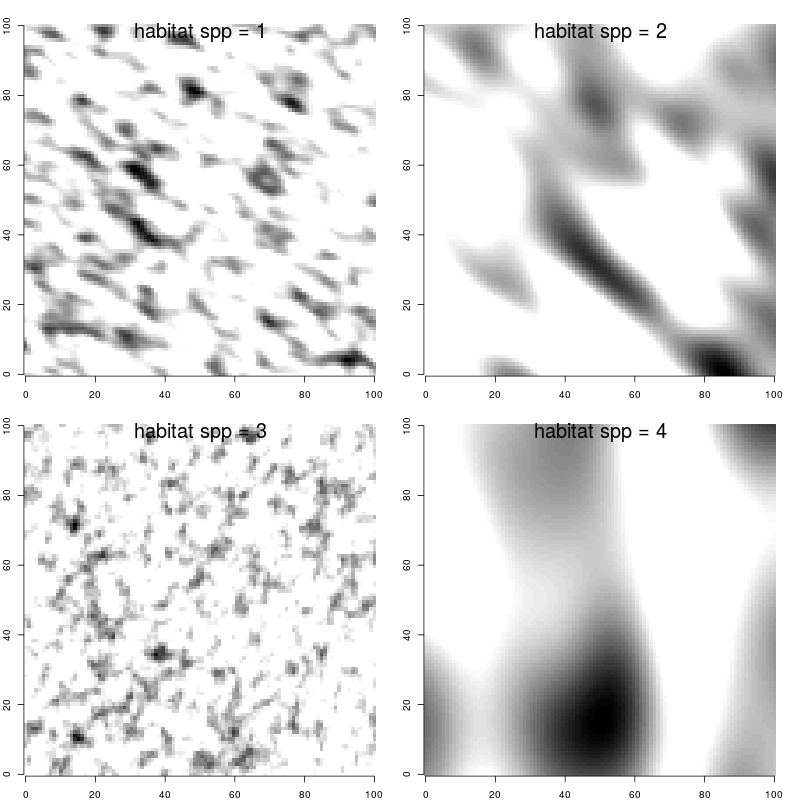
\includegraphics[width = \linewidth]{../tests/plots/habitat}
		\caption{habitat}
\end{figure}	

\begin{figure}[!ht]
	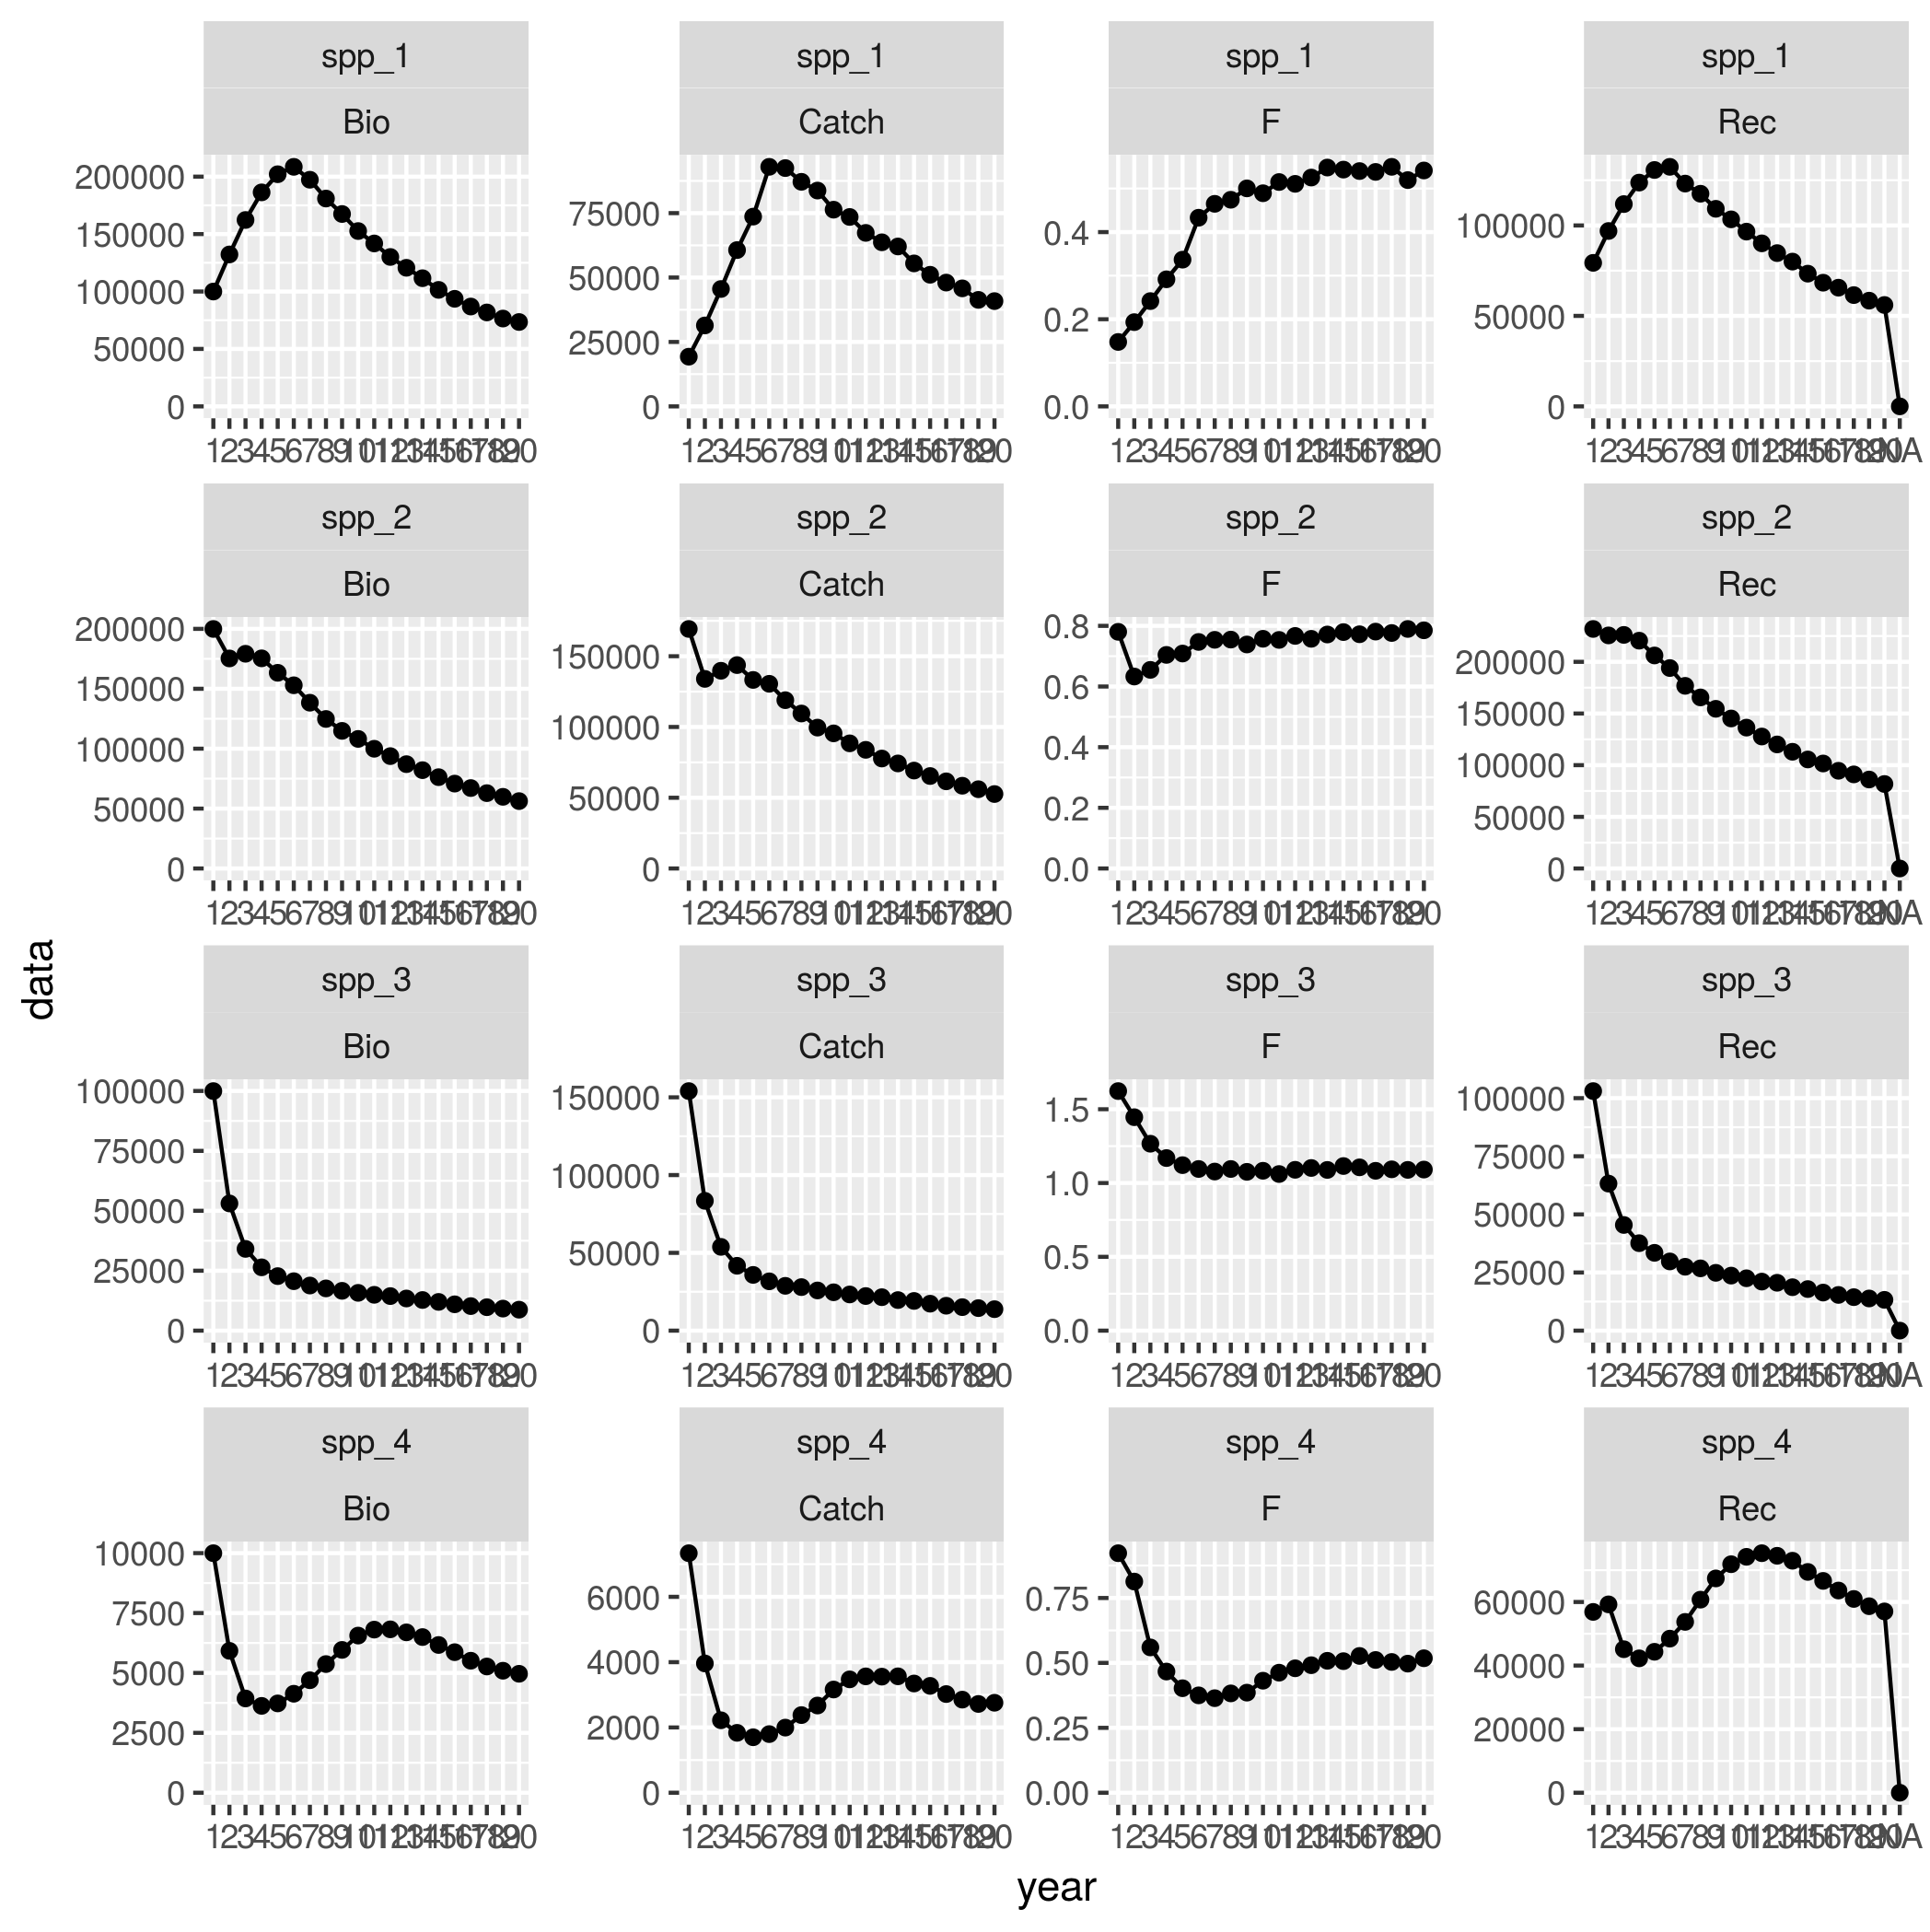
\includegraphics[width = \linewidth]{../tests/plots/annual_summary}
		\caption{Annual Summmary}
\end{figure}	

\begin{figure}[!ht]
	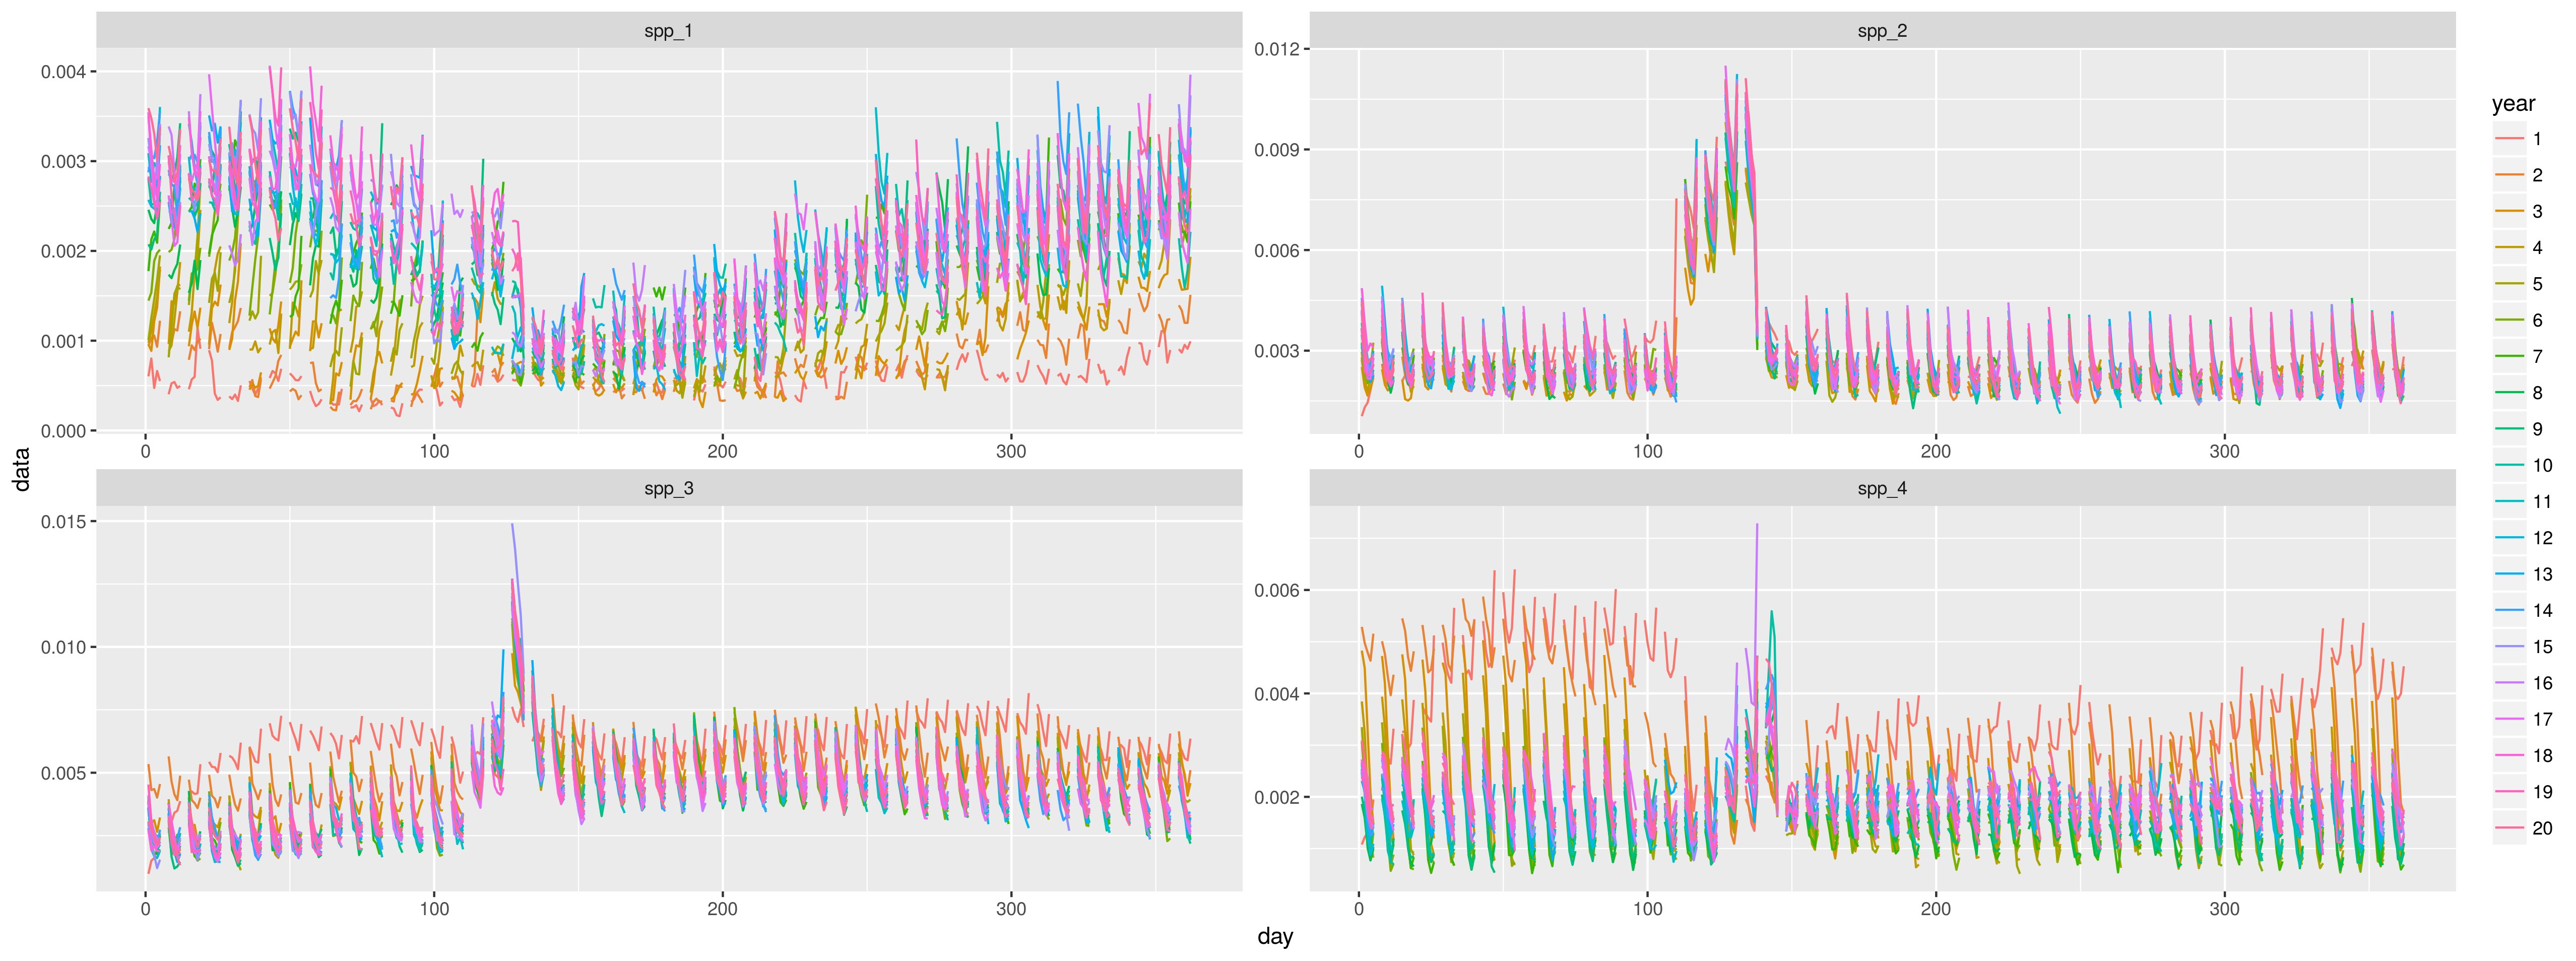
\includegraphics[width = \linewidth]{../tests/plots/fDynamics}
		\caption{f dynamics}
\end{figure}	

\begin{figure}[!ht]
	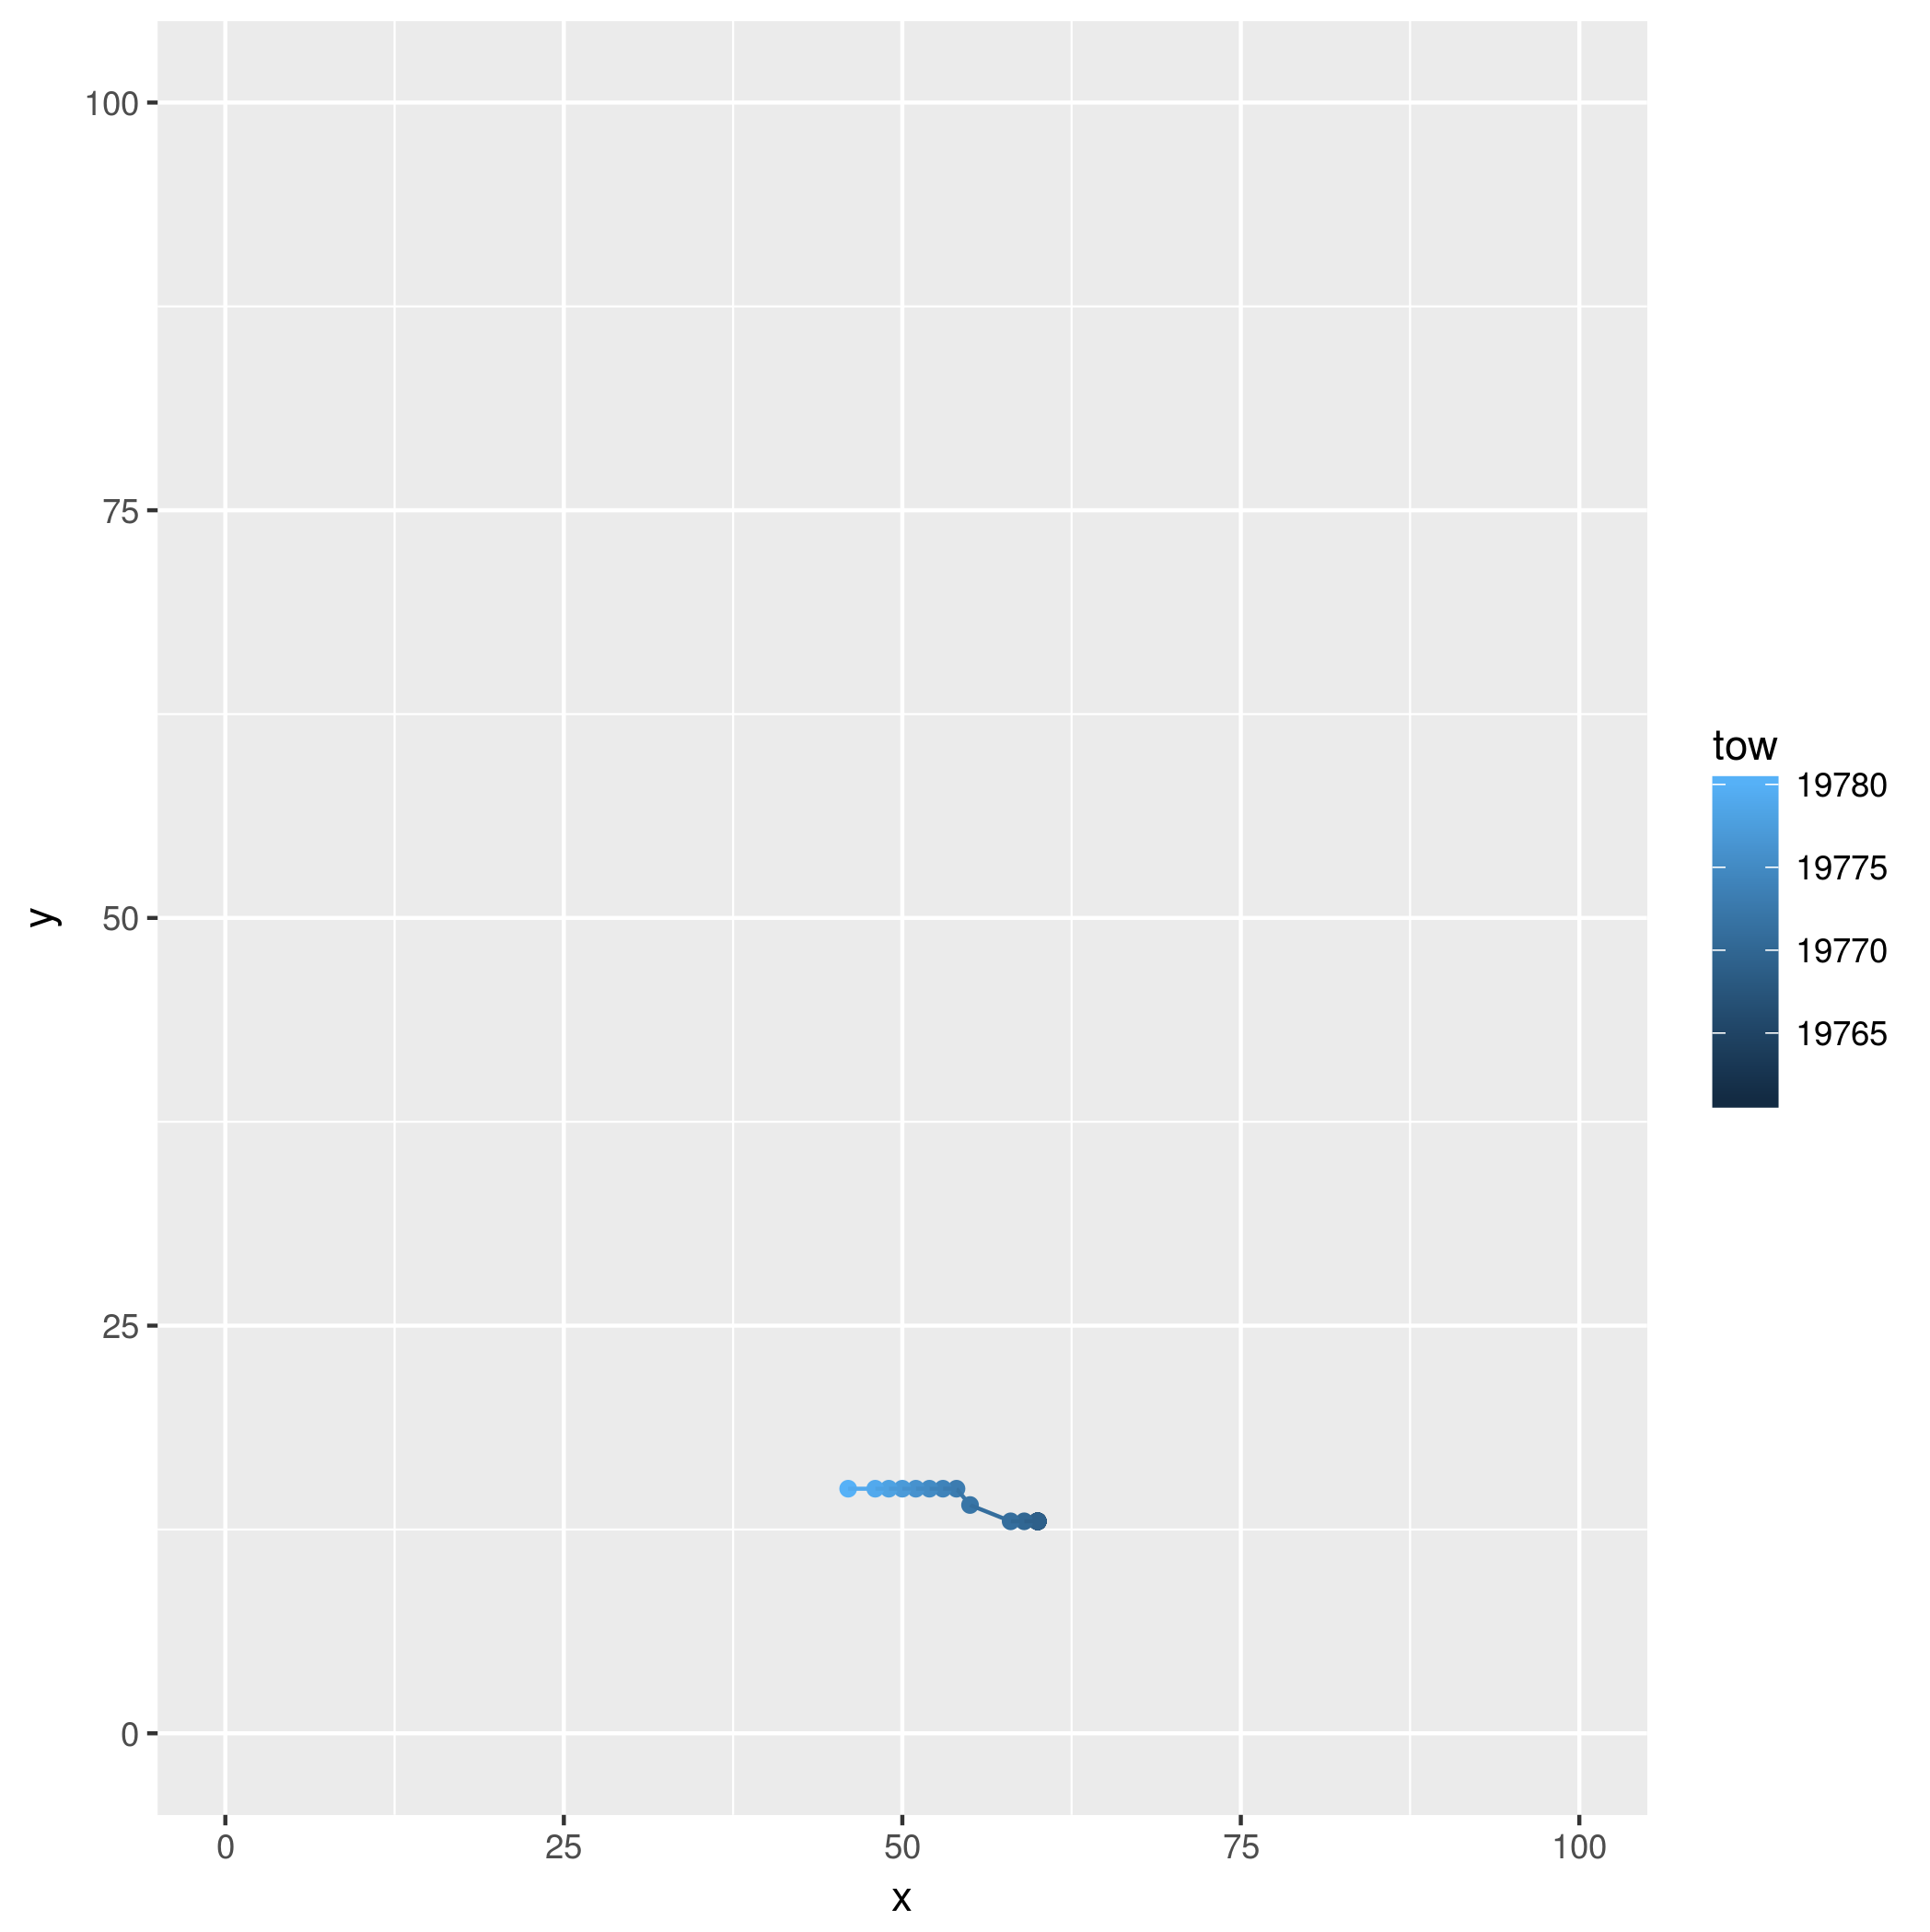
\includegraphics[width = \linewidth]{../tests/plots/vessel_move}
		\caption{vessel movement}
\end{figure}	

\begin{figure}[!ht]
	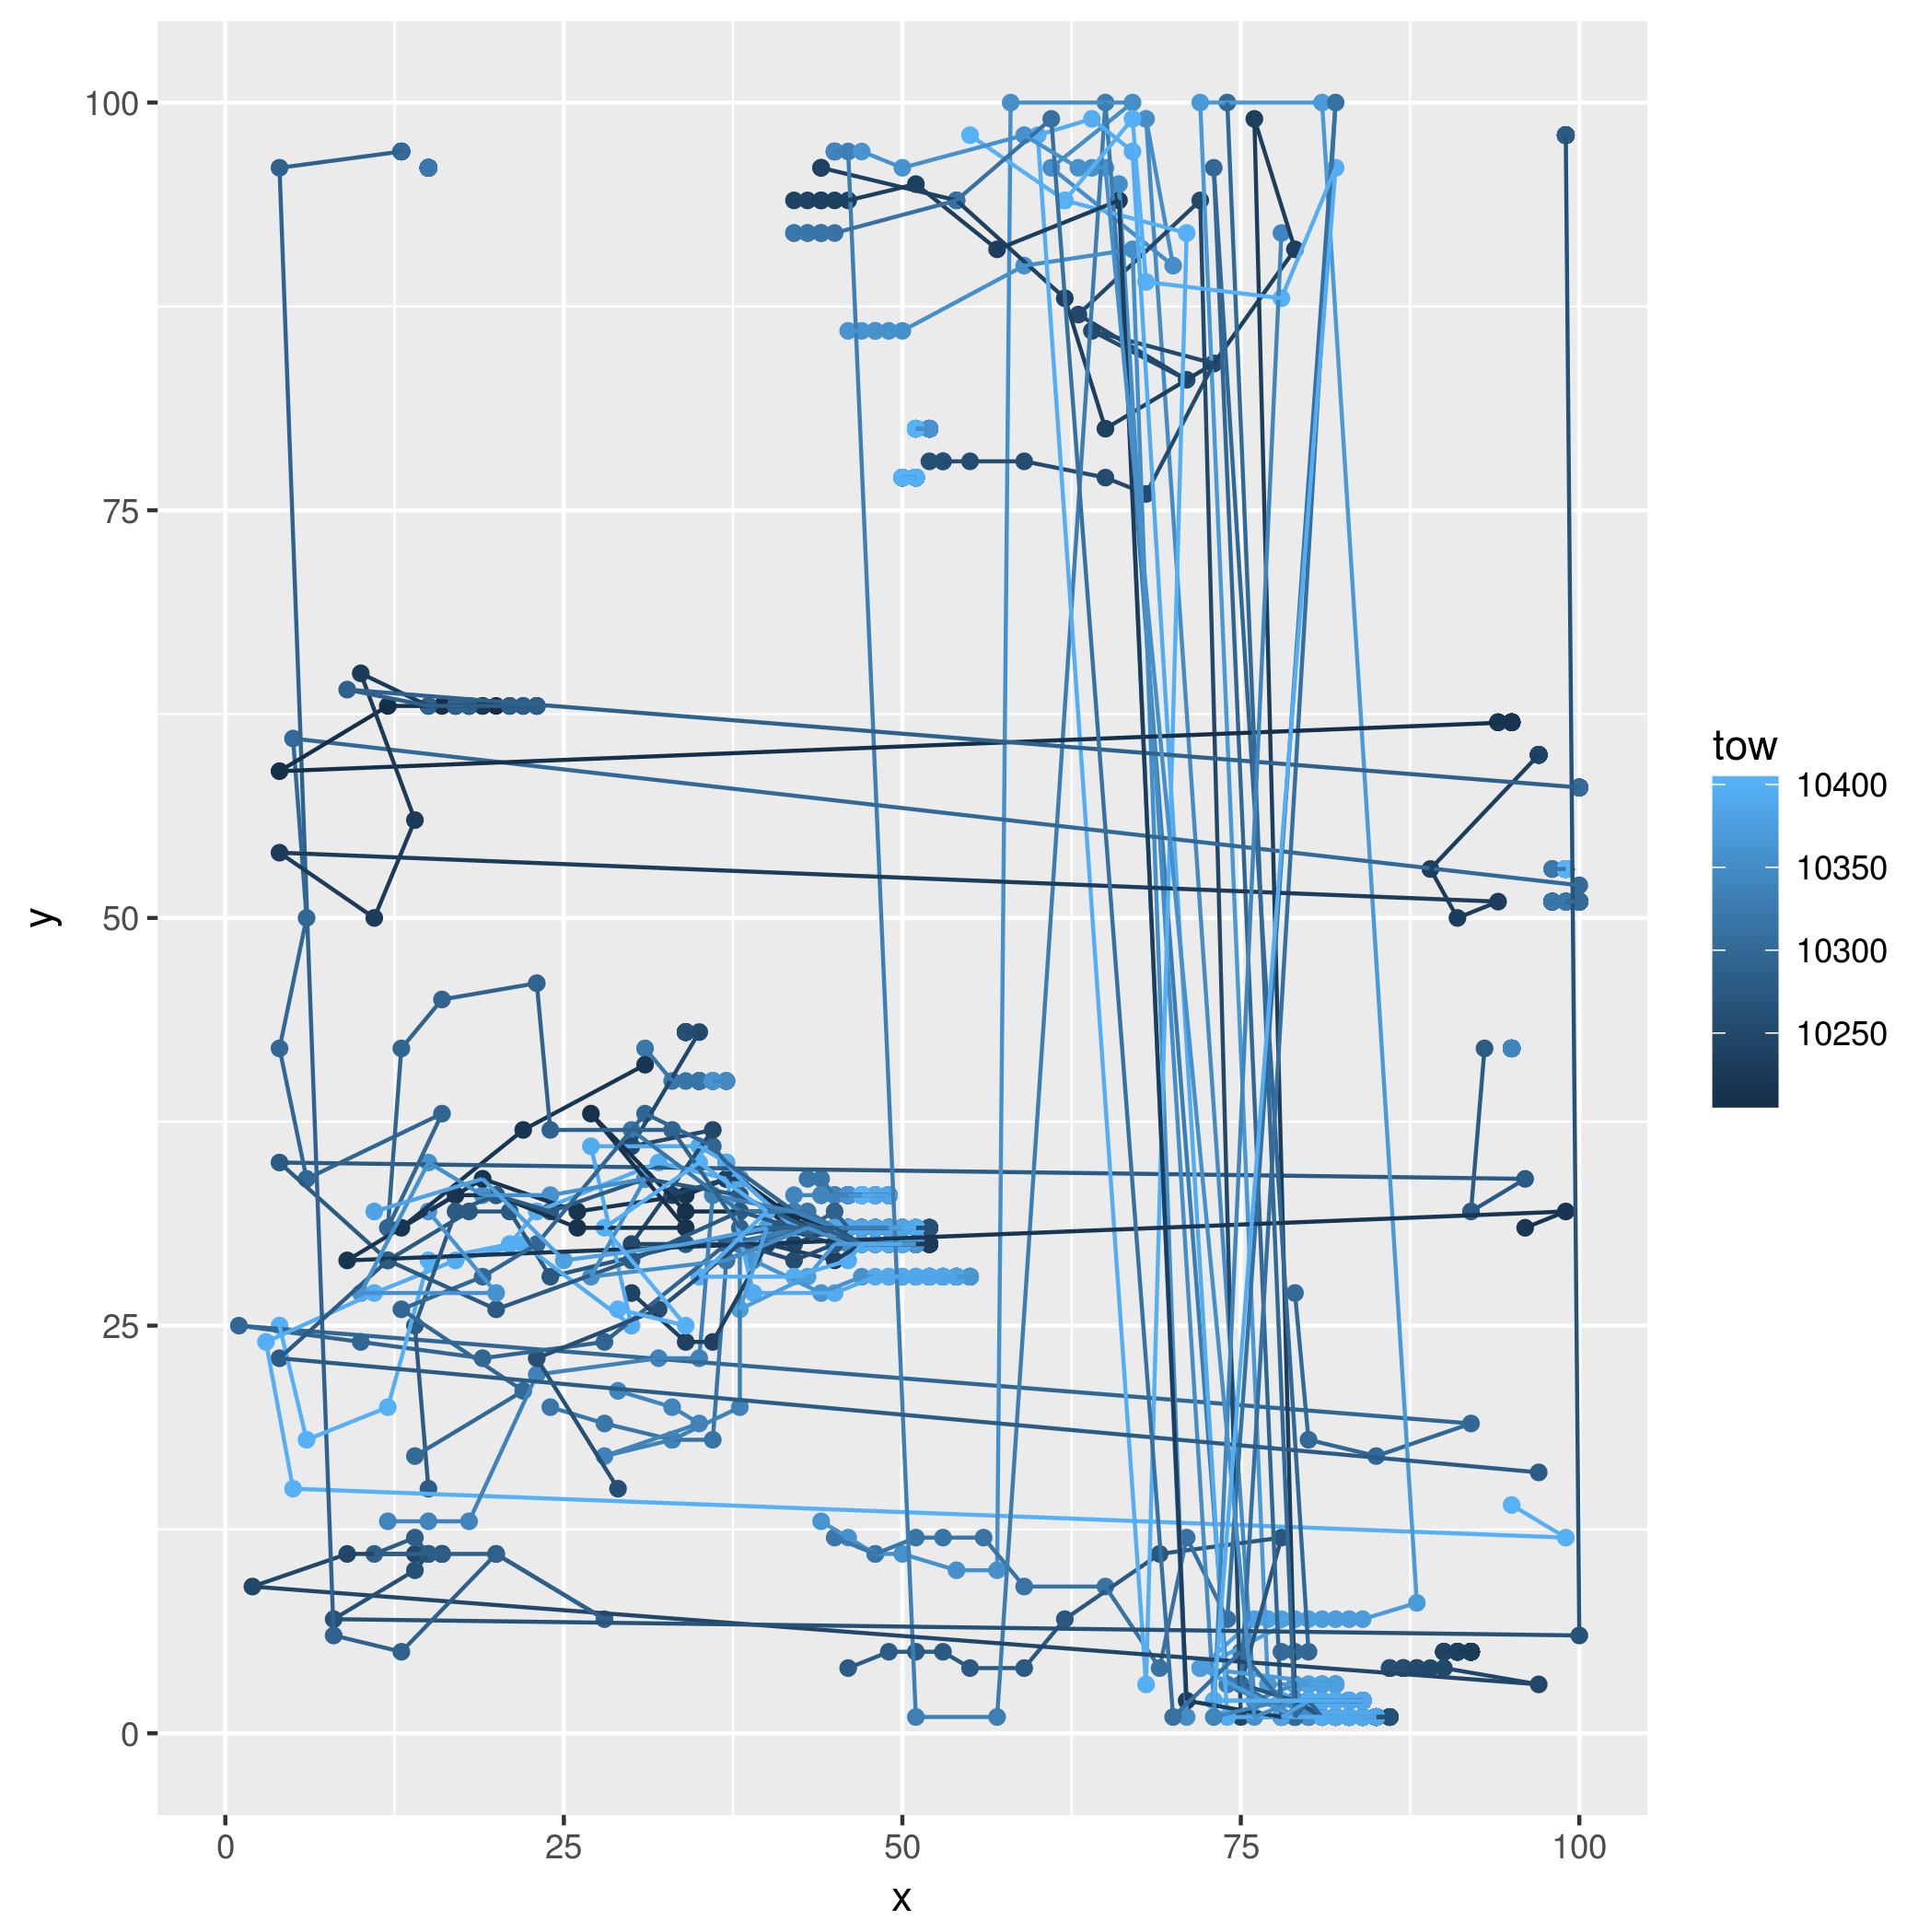
\includegraphics[width = \linewidth]{../tests/plots/vessel_multi_move}
		\caption{vessel movement multi}
\end{figure}	

\begin{figure}[!ht]
	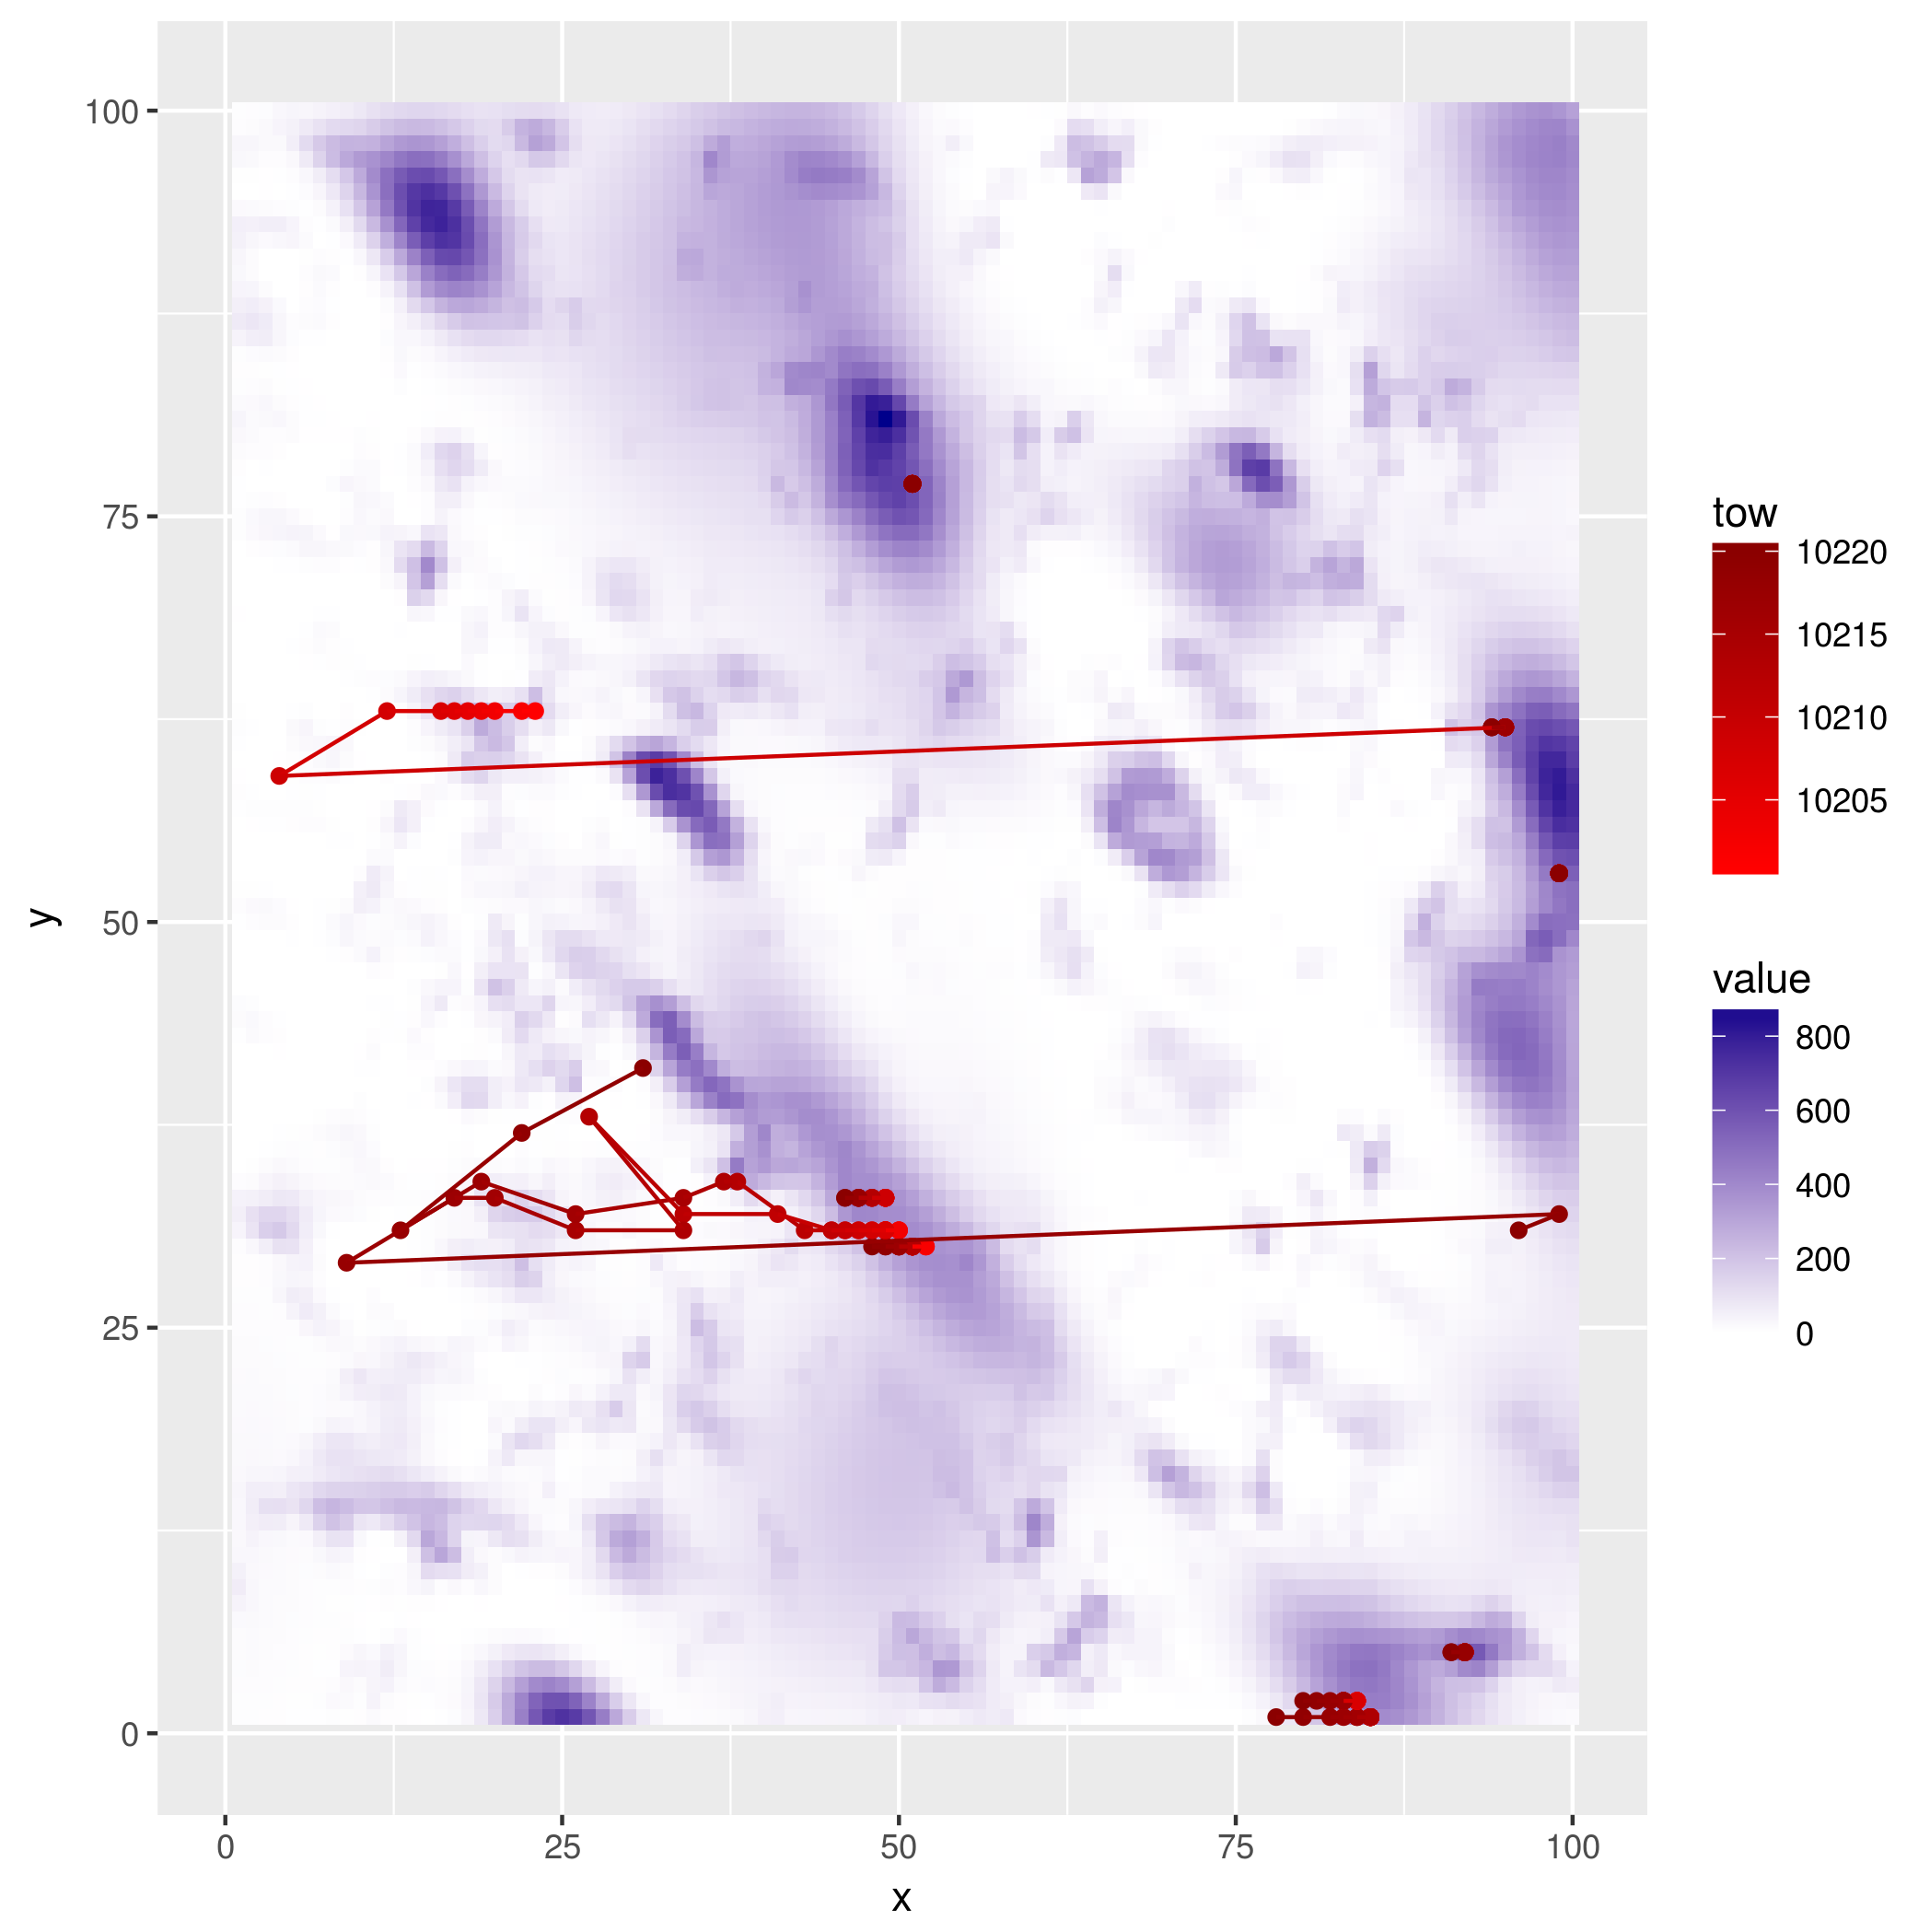
\includegraphics[width = \linewidth]{../tests/plots/vessel_move_value}
		\caption{vessel movement value}
\end{figure}	

\begin{figure}[!ht]
	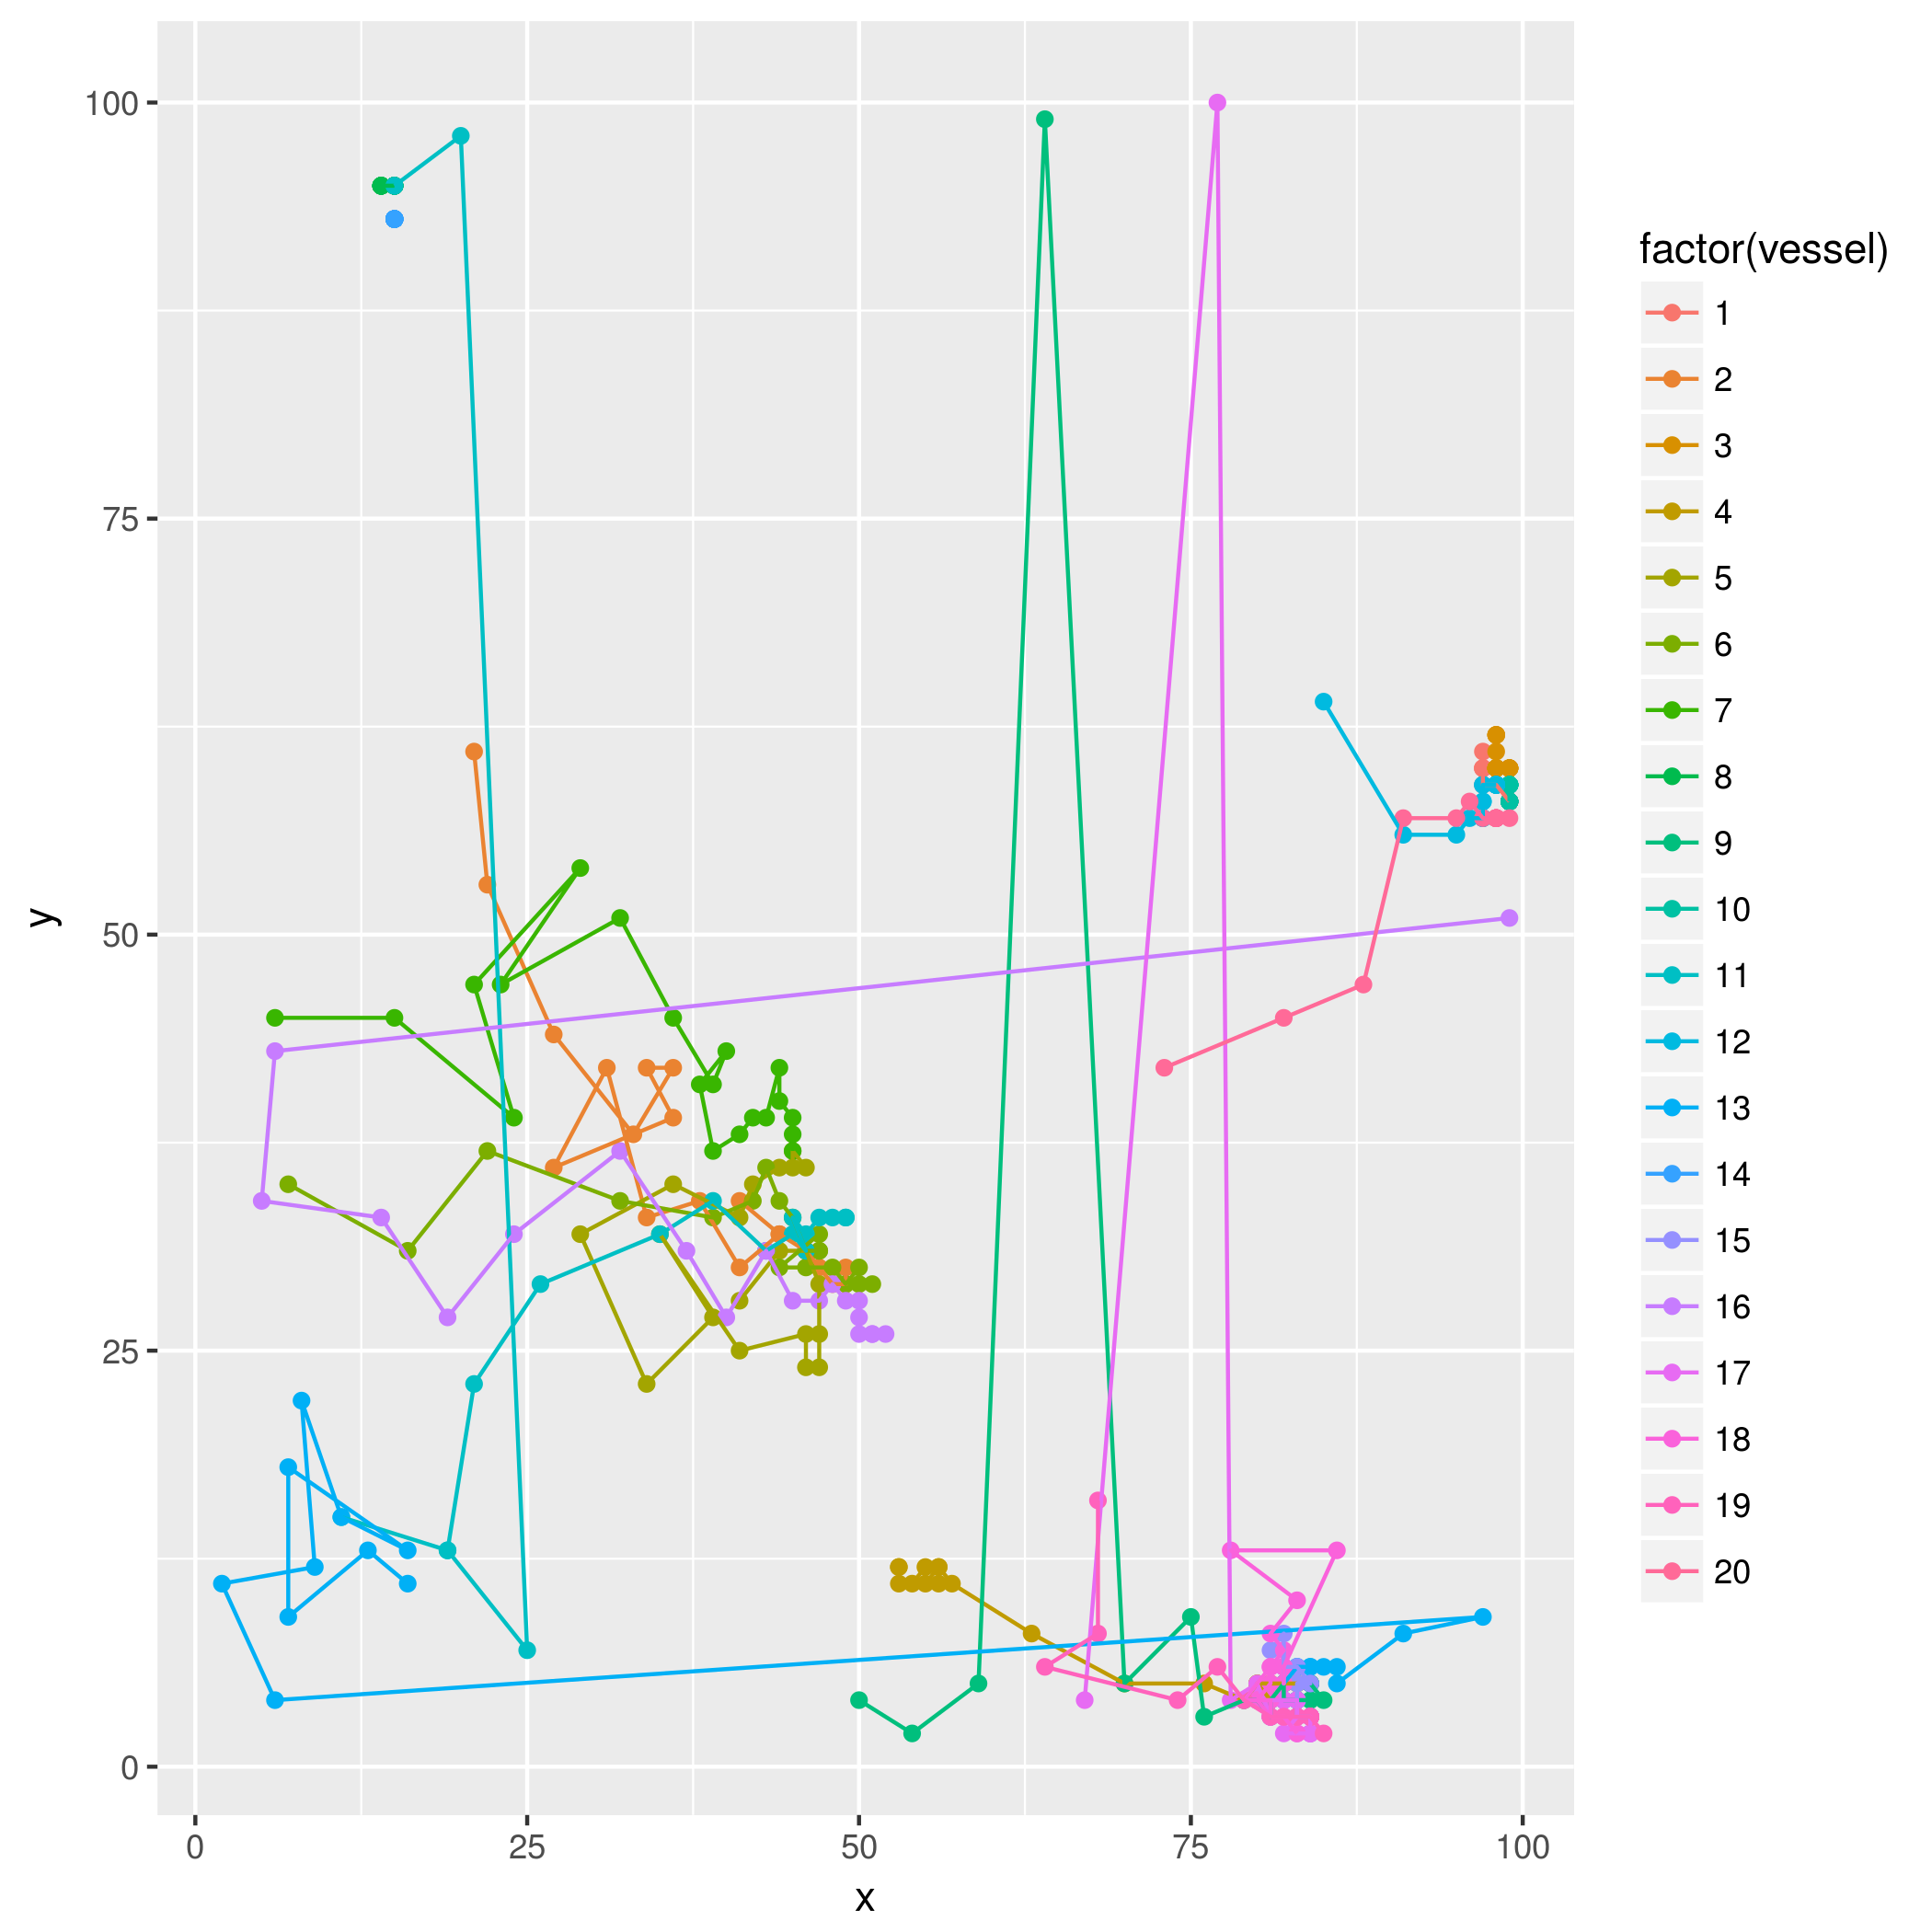
\includegraphics[width = \linewidth]{../tests/plots/fleet_moves}
		\caption{fleet movement}
\end{figure}	

\begin{figure}[!ht]
	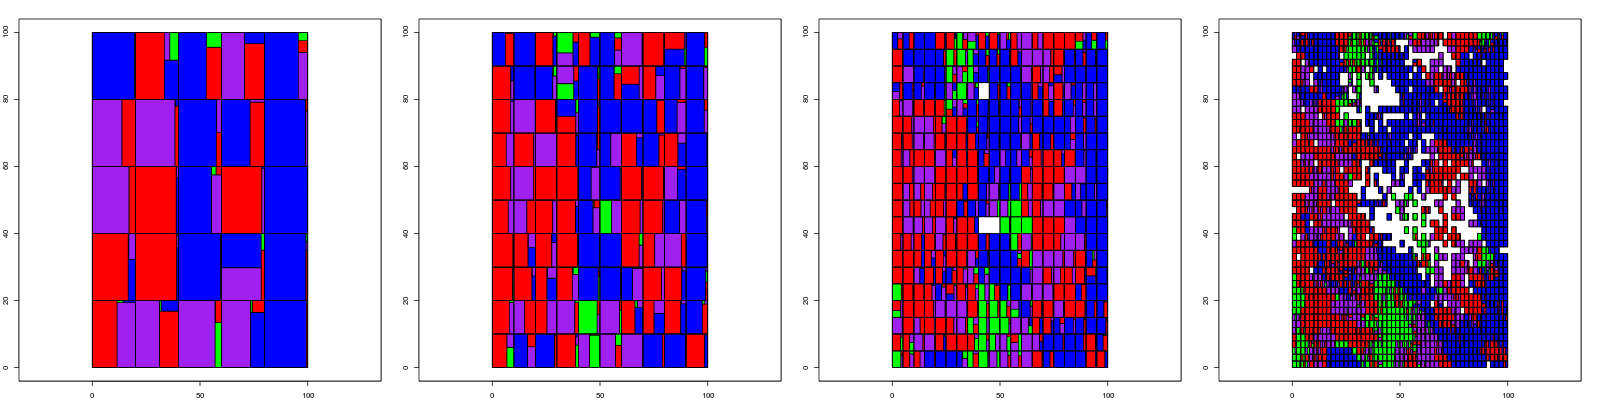
\includegraphics[width = \linewidth]{../tests/plots/catch_comp}
		\caption{spatial catch composition}
\end{figure}	

\begin{figure}[!ht]
	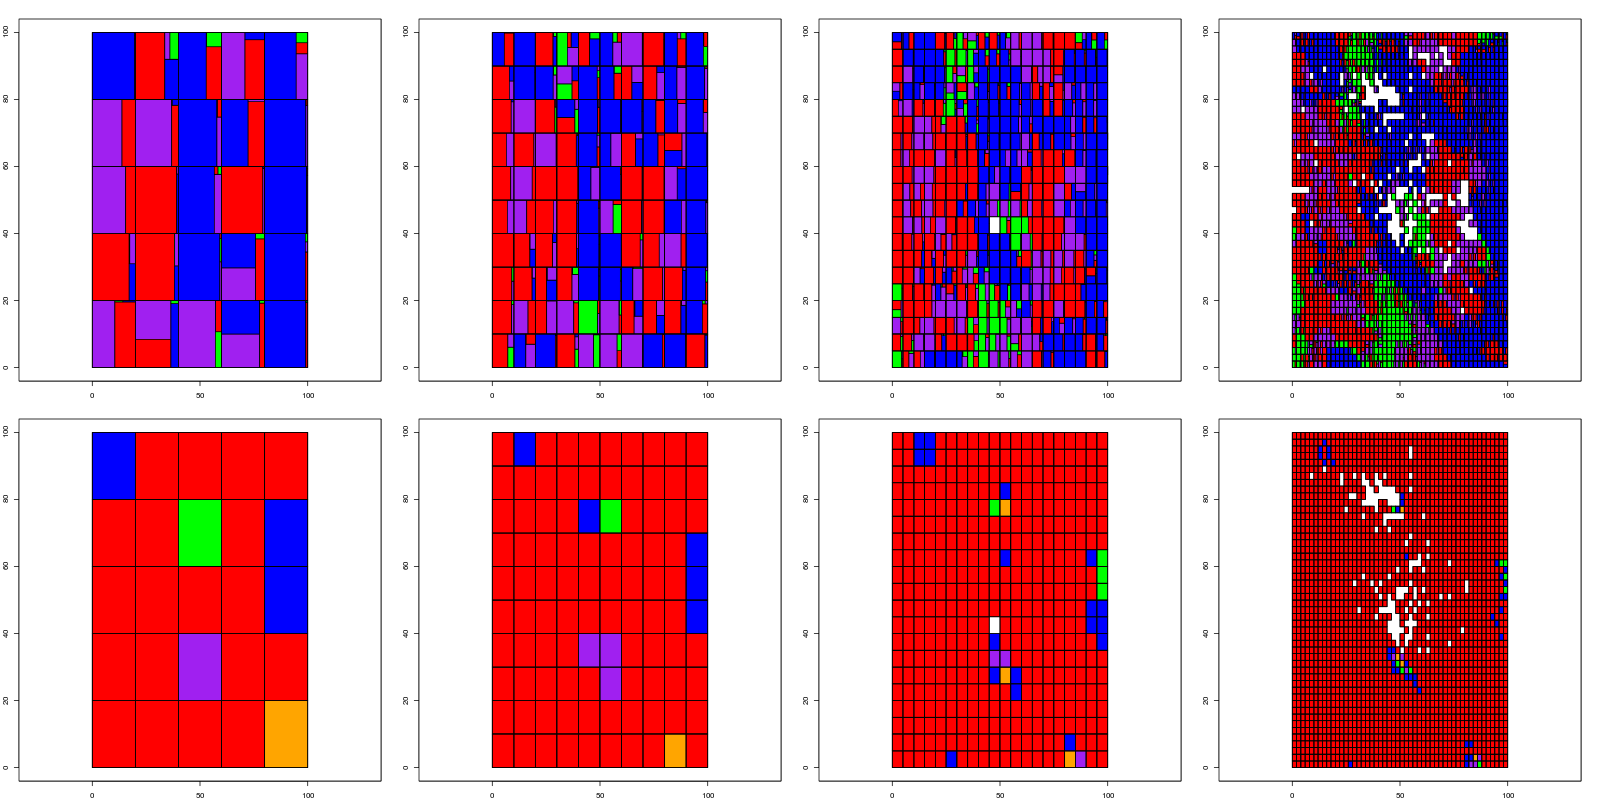
\includegraphics[width = \linewidth]{../tests/plots/catch_comp_clusters}
		\caption{spatial catch composition with clustering}
\end{figure}	

\begin{figure}[!ht]
	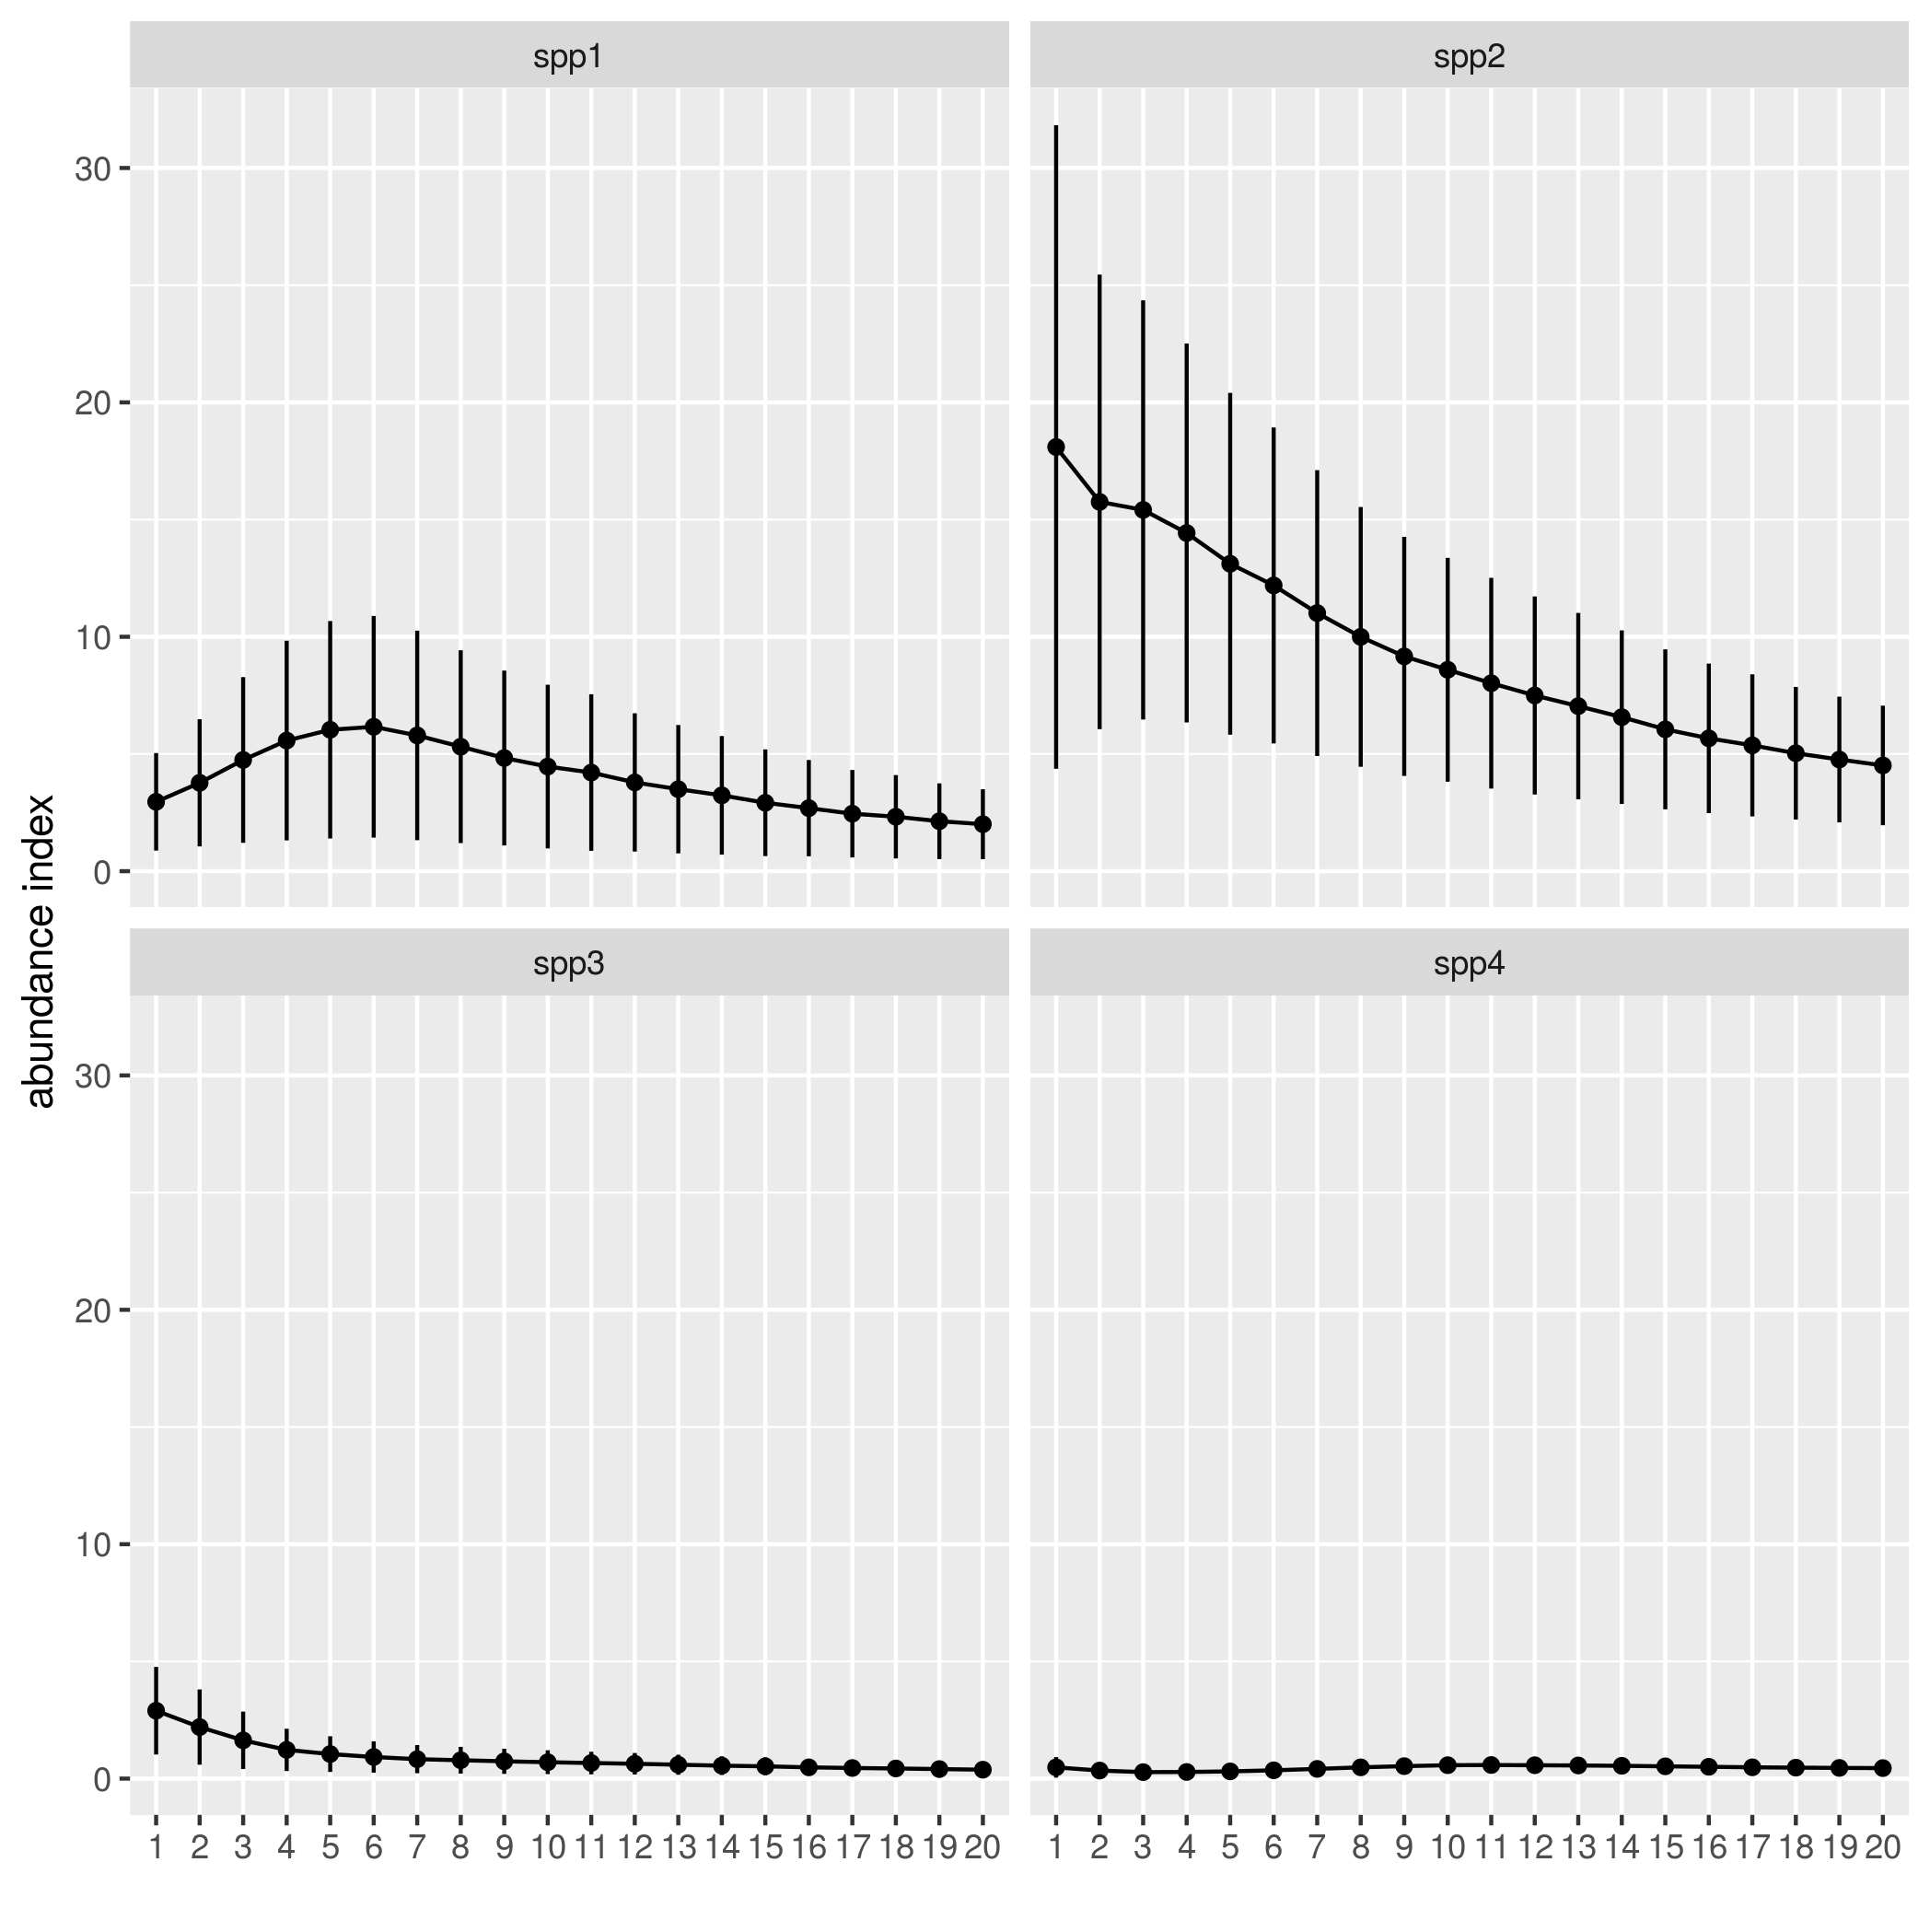
\includegraphics[width = \linewidth]{../tests/plots/survey_index}
		\caption{survey index}
\end{figure}	

\begin{figure}[!ht]
	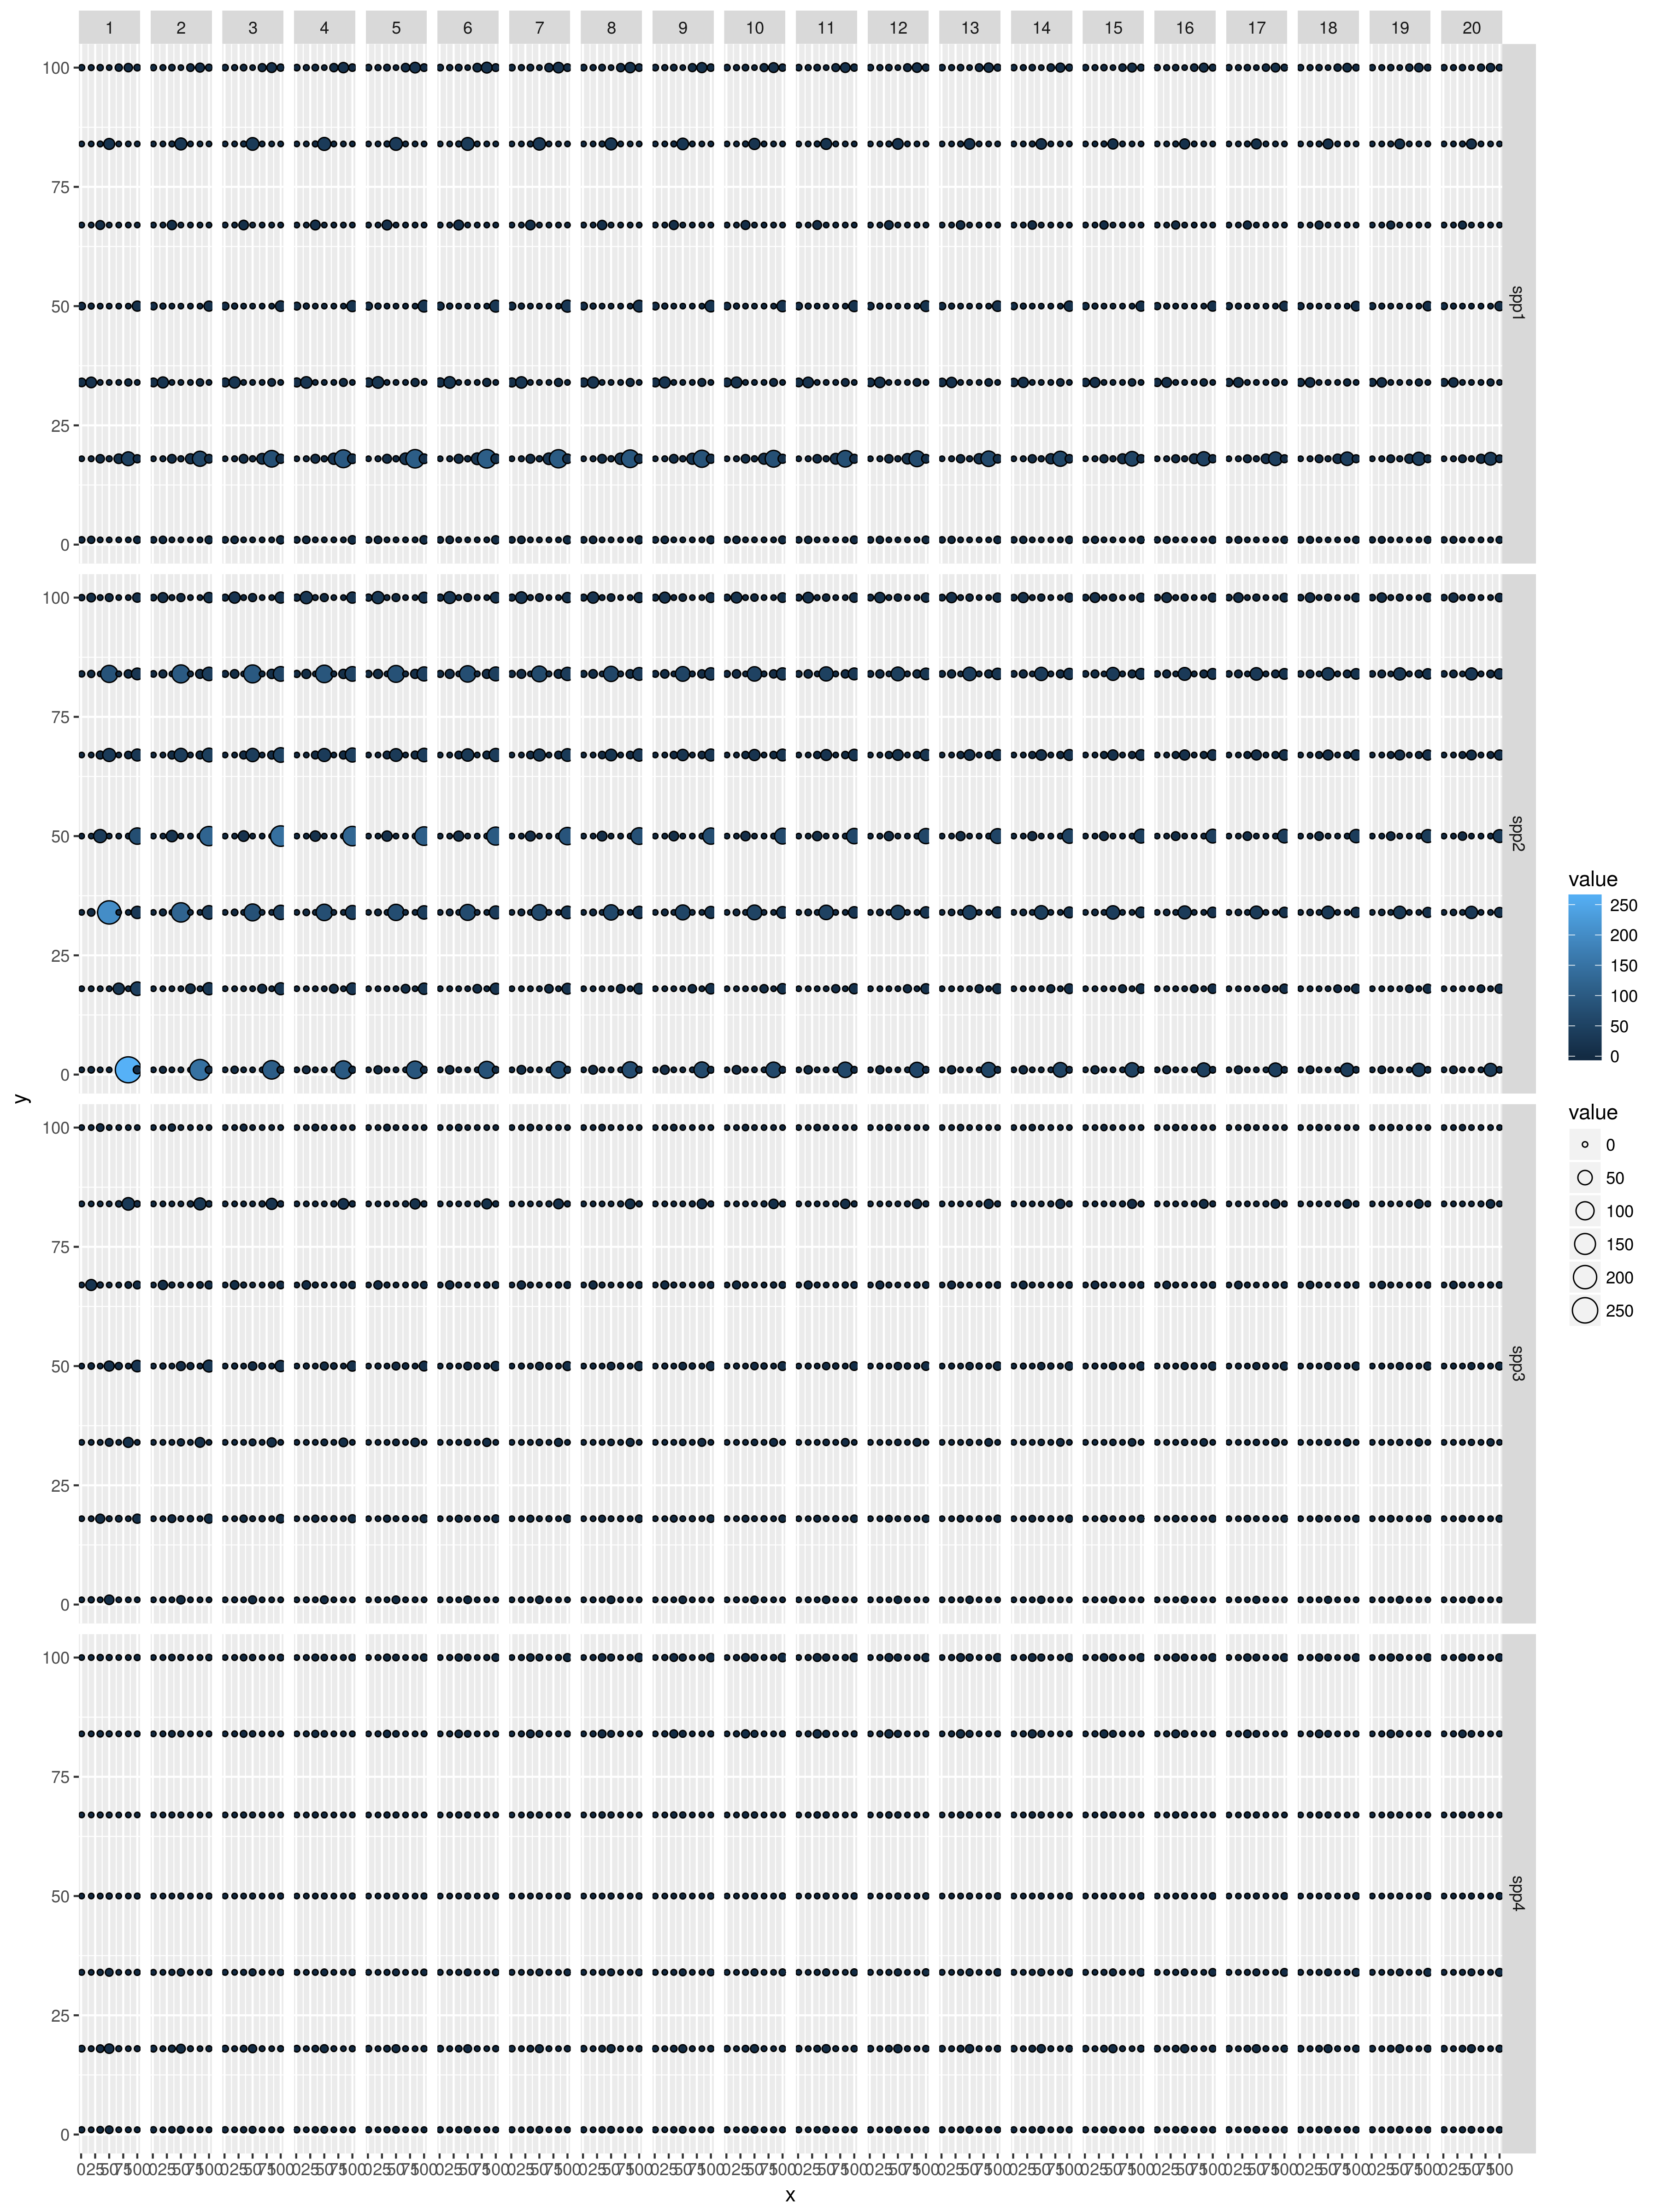
\includegraphics[width = \linewidth]{../tests/plots/spatial_survey}
		\caption{survey spatial abundance}
\end{figure}	

\begin{figure}[!ht]
	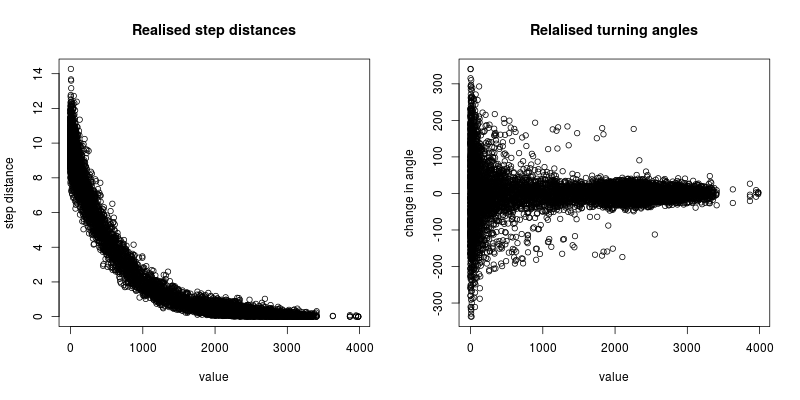
\includegraphics[width = \linewidth]{../tests/plots/step_function}
		\caption{Realised step function}
\end{figure}	





\newpage

\section*{Abbreviations} Detail any unusual ones used.

\section*{Acknowledgements} those providing help during the research..

\section*{Funding} This work was supported by the MARES doctoral training
program; and the Centre for Environment, Fisheries and Aquaculture Science
seedcorn program.

\section*{References}

\bibliography{simulation_framework}

\end{document}
